% Format papiru A4 je pozadavkem fakulty. Trida diploma predava velikost papiru
% tride book az po jejim nacteni, takze na distribucich s vychozim formatem
% letter (MiKTeX) vznikne dokument v nespravnem formatu. Nasledujici radek
% predava volbu vcas.
\PassOptionsToClass{a4paper}{book}

% Nejprve uvedeme tridu dokumentu s volbami
\documentclass[czech,bachelor]{diploma}
% Dalsi doplnujici baliky maker
\usepackage[autostyle=true,czech=quotes]{csquotes} % korektni sazba uvozovek, podpora pro balik biblatex
\usepackage[backend=biber, style=iso-numeric, alldates=iso]{biblatex} % bibliografie
\usepackage{dcolumn} % sloupce tabulky s ciselnymi hodnotami
\usepackage{subfig} % makra pro "podobrazky" a "podtabulky"
\usepackage[cpp]{diplomalst}
\lstset{breaklines=true} % dlouhe radky kodu v prilohach zalomit misto preteceni okraje
\usepackage{tikz} % blokova schemata
\usetikzlibrary{fit,arrows.meta}
\usepackage{pgfplots} % grafy z namerenych dat
\pgfplotsset{compat=1.18}
% Adresy a nazvy v neproporcionalnim pismu nelze delit; radeji mirne roztahnout mezery nez pretect okraj
\setlength{\emergencystretch}{2em}

% Zadame pozadovane vstupy pro generovani titulnich stran.
\ThesisAuthor{Mikhail Mukanov}

\ThesisSupervisor{Ing. Pavel Nevlud}

\CzechThesisTitle{Přenosné zařízení pro testování a monitorování sítí}

\EnglishThesisTitle{Portable Device for Testing and Monitoring Networks}

\SubmissionYear{2027}

\ThesisAssignmentFileName{ThesisSpecification_MUK0015_vsboee250462E0.pdf}

% Pokud nechceme nikomu dekovat makro zapoznamkujeme.
\Acknowledgement{Rád bych na tomto místě poděkoval všem, kteří mi s prací pomohli, protože bez nich by tato práce nevznikla.}

\CzechAbstract{Tato bakalářská práce se zabývá návrhem a realizací přenosného zařízení pro testování a monitorování počítačových sítí. Zařízení je postaveno na jednodeskovém počítači Raspberry Pi s dotykovým displejem, dvěma externími síťovými adaptéry a akumulátorovým modulem a ovládá se bez připojeného počítače. Oba testovací porty jsou logicky odděleny jmennými prostory jádra Linux, takže přístroj může jedním portem provoz generovat a druhým jej nezávisle analyzovat. Zařízení obsahuje analyzátor provozu protokolů IPv4 a IPv6 se statistikami, rozborem rámců a filtry vyhodnocovanými v jádře, generátor paketů, měření zpoždění, propustnosti, ztrátovosti a rozptylu zpoždění nástrojem iperf3 včetně rozmítání velikostí rámce, audit zpráv Router Advertisement a vyhledání sousedů protokolu IPv6. Přesnost analyzátoru byla ověřena nezávislým přepočtem zachyceného provozu a měření proběhla na propojce mezi porty i proti počítačům se systémy Linux a Windows. Práce vymezuje i meze použité platformy, zejména propustnost omezenou sběrnicí USB 2.0 na přibližně 276 Mbit/s. V typickém provozu vydrží přístroj z akumulátoru téměř sedm hodin.}

\CzechKeywords{počítačové sítě; monitorování sítě; generování provozu; analyzátor provozu; Raspberry Pi; Network Namespaces; IPv4; IPv6; propustnost; ztrátovost}

\EnglishAbstract{This bachelor thesis deals with the design and implementation of a portable device for testing and monitoring computer networks. The device is built on a Raspberry Pi single-board computer with a touch screen, two external network adapters and a battery module, and it is operated without a connected computer. Both test ports are logically isolated by Linux network namespaces, so that the device can generate traffic on one port and analyse it independently on the other. The device contains an IPv4 and IPv6 traffic analyser with statistics, frame decoding and filters evaluated in the kernel, a packet generator, measurement of delay, throughput, packet loss and jitter with iperf3 including a sweep over frame sizes, an audit of Router Advertisement messages and IPv6 neighbour discovery. The accuracy of the analyser was verified by an independent recount of the captured traffic, and the measurements were carried out both over a cable between the two ports and against computers running Linux and Windows. The thesis also defines the limits of the platform used, in particular the throughput limited by the USB 2.0 bus to about 276 Mbit/s. In typical operation the device runs on its battery for almost seven hours.}

\EnglishKeywords{computer networks; network monitoring; traffic generation; traffic analyser; Raspberry Pi; network namespaces; IPv4; IPv6; throughput; packet loss}

\AddAcronym{ARP}{Address Resolution Protocol}
\AddAcronym{BPF}{Berkeley Packet Filter}
\AddAcronym{CSV}{Comma-Separated Values}
\AddAcronym{DHCP}{Dynamic Host Configuration Protocol}
\AddAcronym{DNS}{Domain Name System}
\AddAcronym{EUI-64}{64-bit Extended Unique Identifier}
\AddAcronym{GPIO}{General-Purpose Input/Output}
\AddAcronym{HDMI}{High-Definition Multimedia Interface}
\AddAcronym{I2C}{Inter-Integrated Circuit}
\AddAcronym{ICMP}{Internet Control Message Protocol}
\AddAcronym{IP}{Internet Protocol}
\AddAcronym{JSON}{JavaScript Object Notation}
\AddAcronym{LAN}{Local Area Network}
\AddAcronym{MTU}{Maximum Transmission Unit}
\AddAcronym{NTP}{Network Time Protocol}
\AddAcronym{RFC}{Request for Comments}
\AddAcronym{TCP}{Transmission Control Protocol}
\AddAcronym{UDP}{User Datagram Protocol}
\AddAcronym{USB}{Universal Serial Bus}
\AddAcronym{VLAN}{Virtual Local Area Network}

\addbibresource{literature.bib}


% Novy druh tabulkoveho sloupce, ve kterem jsou cisla zarovnana podle desetinne carky
\newcolumntype{d}[1]{D{,}{,}{#1}}


% Zacatek dokumentu
\begin{document}

% Nechame vysazet titulni strany.
\MakeTitlePages

% Jsou v praci obrazky? Pokud ano vysazime jejich seznam a odstrankujeme.
% Pokud ne smazeme nasledujici dve makra.
\listoffigures
\clearpage

% Jsou v praci tabulky? Pokud ano vysazime jejich seznam a odstrankujeme.
% Pokud ne smazeme nasledujici dve makra.
\listoftables
\clearpage

% A nasleduje text zaverecne prace.
\chapter{Úvod}
\label{sec:introduction}

Počítačové sítě jsou dnes základní infrastrukturou, na jejíž spolehlivosti závisí provoz institucí i výrobních podniků. S rostoucím počtem připojených zařízení a s postupným zaváděním protokolu IPv6 vedle zavedeného protokolu IPv4 roste i složitost úloh, které musí správce sítě řešit přímo na místě. Otázky bývají přitom velmi konkrétní: zda je zásuvka v místnosti skutečně propojena s rozvaděčem, jakou propustnost daná linka nabízí, která zařízení se v segmentu nacházejí a zda na nich neběží služby, které by běžet neměly.

Odpověď na tyto otázky vyžaduje měření na místě. Právě zde naráží běžně dostupná řešení na svá omezení. Komerční příruční testery jsou ergonomické, ale uzavřené, takže rozsah jejich funkcí je pevně dán výrobcem a vlastní testovací postup do nich doplnit nelze. Notebook s otevřenými nástroji je naopak plně flexibilní, avšak v rozvaděči nebo pod stolem se s ním pracuje obtížně a před každým měřením vyžaduje ruční nastavení. Pokusí-li se navíc technik připojit do téhož segmentu dvěma rozhraními, aby mohl současně naslouchat provozu a generovat zátěž, narazí na konflikt ve směrovacích tabulkách operačního systému, který výsledky měření nenápadně zkreslí.

Cílem této bakalářské práce je navrhnout a realizovat přenosné zařízení pro testování a monitorování počítačových sítí, které spojuje otevřenost softwarového řešení s ergonomií samostatného přístroje. Prototyp je postaven na jednodeskovém počítači Raspberry Pi, je vybaven dotykovým displejem, vlastní řídicí aplikací a akumulátorem, takže jej lze ovládat bez připojeného počítače, bez fyzické klávesnice a bez síťového zdroje. Obsahuje generátor i analyzátor provozu, měří zpoždění, propustnost, ztrátovost a rozptyl zpoždění a umožňuje mapování segmentu i bezpečnostní průzkum, a to shodně pro protokoly IPv4 a IPv6.

Klíčovým technickým prvkem návrhu je logické oddělení dvou testovacích rozhraní pomocí technologie Linux Network Namespaces. Toto oddělení zajišťuje, že generovaná zátěž neovlivňuje statistiky zachycené naslouchajícím rozhraním, a je vynuceno přímo jádrem operačního systému, nikoli pouze konfigurační kázní obsluhy. Druhou oblastí, které je věnována zvýšená pozornost, je automatická konfigurace adres protokolu IPv6, neboť právě na ní závisí, zda přístroj dokáže navázat spojení se stanicí, na níž není nic předem nastaveno.

Text práce je rozdělen do čtyř kapitol. Po tomto úvodu následuje kapitola \ref{sec:teorie}, která shrnuje teoretická východiska: rozdíly mezi protokoly síťové vrstvy, adresaci a automatickou konfiguraci protokolu IPv6, generování síťového provozu a měření jeho parametrů, nástroje pro monitorování a audit provozu a architekturu jmenných prostorů. Její závěrečná část porovnává existující řešení a formuluje požadavky na navrhované zařízení. Kapitola \ref{sec:realizace} popisuje návrh přístroje po hardwarové i softwarové stránce, realizaci generátoru a analyzátoru provozu a zhodnocení výsledků ověřených laboratorním měřením. Závěr práce shrnuje dosažené výsledky, vymezuje vlastní přínos autora a naznačuje směry dalšího vývoje prototypu.
\chapter{Teoretická východiska a analýza problematiky}
\label{sec:teorie}

Tato kapitola se věnuje teoretickým základům, na kterých je postaveno navržené testovací a monitorovací zařízení. Porozumění těmto konceptům je nezbytné pro správnou interpretaci dat získaných při analýze sítě.

\section{Protokoly síťové vrstvy a jejich výkonnostní rozdíly}
\label{sec:ipv4_ipv6}

Moderní počítačové sítě spoléhají na koexistenci protokolů IPv4 a IPv6 \cite{nastase2024}. Obě verze plní na síťové vrstvě tutéž úlohu, tedy adresování stanic a doručení paketu mezi sítěmi, liší se však natolik, že měřicí přístroj musí každou z nich obsluhovat samostatně. Souběžný provoz obou protokolů na jednom rozhraní, označovaný jako dvojí zásobník, je dnes v podnikových sítích běžný, a přenosný analyzátor proto musí umět ověřit funkčnost každé větve zvlášť.

Nejnápadnějším rozdílem je délka adresy, která vzrostla ze 32 na 128~bitů. Změna adresního prostoru ovšem není jediným zásahem do konstrukce protokolu. Hlavička protokolu IPv4 má proměnnou délku od 20 do 60~bajtů, neboť za povinnou částí mohou následovat volitelná pole, a obsahuje mimo jiné vlastní kontrolní součet a trojici polí sloužících k fragmentaci. Hlavička protokolu IPv6 je oproti tomu pevná a měří 40~bajtů \cite{rfc8200}. Veškerá doplňková funkcionalita byla přesunuta do rozšiřujících hlaviček, které se řetězí za základní hlavičku a na jejichž existenci upozorňuje pole Next Header.

Tento návrh má dva důsledky, jež se projeví právě při měření. Předně směrovač na cestě paketu vykonává méně práce: nepočítá znovu kontrolní součet, protože ten byl z hlavičky zcela odstraněn a spoléhá se na zabezpečení na linkové a transportní vrstvě, a nefragmentuje. Fragmentaci smí v protokolu IPv6 provést pouze odesílající stanice, která si k tomu musí předem zjistit nejmenší velikost přenosové jednotky na celé cestě. S tím souvisí požadavek, aby každá linka přenesla paket o velikosti alespoň 1280~bajtů. Druhým důsledkem je, že protokol IPv6 zcela opustil všesměrové vysílání a nahradil je vysíláním skupinovým, což se přímo promítá do způsobu, jakým zařízení v segmentu nacházejí jedno druhé; této otázce je věnována podkapitola \ref{sec:ipv6_adresace}.

Z pohledu měření propustnosti je podstatné, že dvojnásobná velikost základní hlavičky představuje režii, která se odečítá od užitečného zatížení. Při shodné velikosti rámce na linkové vrstvě zbývá na data o dvacet bajtů méně, a naměřená aplikační propustnost proto u protokolu IPv6 vychází nepatrně nižší. Jak dokládá srovnávací měření Tuifaigy a kolektivu \cite{tuifaiga2021}, protokol IPv4 v lokálních sítích skutečně dosahuje o něco vyšší propustnosti a nižší latence než IPv6, a to shodně v prostředí operačních systémů Windows i Linux.

Rozdíl je ovšem třeba interpretovat opatrně. Jeho relativní velikost závisí na tom, jak velké datové jednotky se přenášejí: u dlouhých toků s plnou velikostí rámce jde o jednotky procent, kdežto u provozu složeného z krátkých paketů může být znatelně vyšší. Naměřený rozdíl mezi oběma protokoly proto sám o sobě nevypovídá o kvalitě sítě, nýbrž o vlastnostech protokolu, a při vyhodnocování zátěžových testů popsaných v kapitole \ref{sec:realizace} je nutné jej od případných skutečných závad odlišit.

\section{Adresace a automatická konfigurace protokolu IPv6}
\label{sec:ipv6_adresace}

Rozdíl mezi oběma protokoly se neomezuje na velikost hlavičky. Podstatnější pro přenosný analyzátor je odlišný způsob, jakým se stanice ke své adrese vůbec dostane, neboť právě na něm závisí, zda přístroj dokáže oslovit protistranu bez jakékoli předchozí domluvy s její obsluhou. Této otázce je proto věnována samostatná podkapitola.

Adresa protokolu IPv6 má délku 128~bitů a její struktura je definována adresní architekturou \cite{rfc4291}, samotný protokol pak dokumentem \cite{rfc8200}. Zápis se člení do osmi skupin po čtyřech hexadecimálních číslicích, přičemž nejdelší souvislý úsek nulových skupin lze nahradit dvojicí dvojteček. Pro účely testovacího zařízení jsou podstatné tři kategorie adres. Adresa lokální linky z rozsahu \texttt{fe80::/10} vzniká na každém rozhraní automaticky ve chvíli, kdy je linka zdvižena, a platí pouze v rámci jednoho fyzického segmentu. Adresa globálního dosahu je směrovatelná v celém Internetu. Mezi nimi stojí kategorie jedinečných lokálních adres, která je pro navržené zařízení nejzajímavější.

Jedinečné lokální adresy jsou vymezeny prefixem \texttt{fc00::/7}, přičemž osmý bit rozlišuje způsob přidělení; při jeho nastavení, tedy pro prefix \texttt{fd00::/8}, si organizace generuje čtyřicetibitový identifikátor sama pseudonáhodným postupem \cite{rfc4193}. Takto vzniklý prefix je s velmi vysokou pravděpodobností jedinečný, není směrovatelný v Internetu a nezávisí na žádném poskytovateli připojení. Právě tyto vlastnosti odpovídají povaze přenosného analyzátoru, který pracuje v uzavřeném testovacím segmentu, nemá trvalé připojení k Internetu a jehož adresní plán nesmí kolidovat s adresami sítě, do níž je přístroj dočasně zapojen.

Druhou polovinu adresy tvoří identifikátor rozhraní o délce 64~bitů. Jeden ze způsobů jeho odvození, popsaný v adresní architektuře \cite{rfc4291}, vychází z fyzické adresy rozhraní a označuje se jako EUI-64. Osmačtyřicetibitová adresa se rozdělí na dvě poloviny, mezi něž se vloží dva bajty s hodnotou \texttt{fffe}, a v prvním bajtu se invertuje sedmý bit rozlišující univerzální a lokální správu. Fyzická adresa \texttt{00:e0:4c:68:02:16} tak vede na identifikátor \texttt{02e0:4cff:fe68:0216}. Tento postup je pro navržené zařízení prakticky významný: adresa protistrany z něj vychází deterministicky, a lze ji tedy dopočítat namísto toho, aby byla zapsána napevno do řídicí aplikace.

Identifikátor odvozený z fyzické adresy má ovšem nevýhodu: prozrazuje hardware stanice a umožňuje ji sledovat, ať se připojí do kterékoli sítě. Současné operační systémy proto častěji používají identifikátor, který je sice pro danou síť stálý, ale z fyzické adresy jej odvodit nelze \cite{rfc7217}, a vedle něj navíc dočasné adresy, které se v pravidelných intervalech mění \cite{rfc8981}. Jedna stanice tak na jednom rozhraní běžně nese několik adres současně, a pokud je tak nastavena, dává pro odchozí komunikaci přednost adrese dočasné \cite{rfc8981}. Pro měřicí přístroj z toho plyne, že protistrana nemusí odpovídat z téže adresy, na kterou byla oslovena, což se v praktické části ukázalo jako podstatné.

O zjišťování sousedů na společné lince se v protokolu IPv6 stará mechanismus Neighbor Discovery \cite{rfc4861}, který nahrazuje protokol ARP známý z protokolu IPv4 a je postaven nad protokolem ICMPv6. Zařízení si jeho prostřednictvím zjišťují vzájemné fyzické adresy, ověřují dosažitelnost sousedů a nacházejí směrovače v segmentu. Pro popisované zařízení jsou klíčové dvě z jeho zpráv. Zprávou Router Solicitation zasílanou na skupinovou adresu všech směrovačů se stanice po zdvižení rozhraní dotazuje, zda je v segmentu přítomen směrovač. Odpovědí je zpráva Router Advertisement, kterou směrovač inzeruje sám sebe a spolu s tím i prefixy platné v daném segmentu. Součástí mechanismu je rovněž detekce duplicitních adres, kterou stanice ověřuje, že jí zvolená adresa není v segmentu již obsazena.

Na zprávě Router Advertisement je postavena bezstavová automatická konfigurace adres \cite{rfc4862}. Stanice si z inzerovaného prefixu a z vlastního identifikátoru rozhraní sestaví úplnou adresu sama, bez jakéhokoli serveru, který by o přidělení vedl evidenci. Zda a jak tuto možnost využije, řídí trojice příznaků nesených ve zprávě, jejichž význam shrnuje Tabulka \ref{tab:priznaky}.

\begin{table}[htbp]
    \caption{Význam příznaků nesených ve zprávě Router Advertisement}
    \label{tab:priznaky}
    \centering
    \begin{tabular}{clp{7.5cm}}
        \hline
        Příznak & Název & Význam pro cílovou stanici \\
        \hline
        M & Managed address configuration & Adresu si stanice vyžádá od serveru DHCPv6 \\
        O & Other configuration & Ostatní údaje, například adresy serverů DNS, získá od serveru DHCPv6 \\
        A & Autonomous address configuration & Z tohoto konkrétního prefixu si stanice smí sestavit adresu sama \\
        \hline
    \end{tabular}
\end{table}

Zásadní je, že příznaky M a O se vztahují k celé zprávě, kdežto příznak A je nesen u každého inzerovaného prefixu zvlášť. Směrovač tedy může v jediné zprávě inzerovat několik prefixů a u každého z nich zvlášť rozhodnout, zda z něj stanice smí odvodit adresu vlastními silami. Obě cesty se přitom nevylučují a v praxi se běžně kombinují, takže jedna stanice může mít současně adresu sestavenou bezstavově a adresu přidělenou serverem.

Stavovou alternativou je protokol DHCPv6 \cite{rfc8415}, který přebírá roli známou z protokolu IPv4: server vede evidenci přidělených adres, váže je na identifikátor klienta a spravuje dobu jejich zapůjčení. Za cenu této evidence poskytuje správci úplnou kontrolu nad tím, která stanice jakou adresu obdrží, a umožňuje předat i další konfigurační údaje.

Rozdíl mezi oběma přístupy je pro přenosné testovací zařízení podstatný. Stanice s protokolem IPv4 bez běžícího klienta DHCP adresu nezíská nikdy, neboť jiný mechanismus protokol nenabízí. Naproti tomu jádro operačního systému s protokolem IPv6 přiděluje adresu lokální linky samočinně a při zdviženém příznaku A sestaví z inzerovaného prefixu i adresu širšího dosahu, aniž by na stanici musela běžet jakákoli služba pro konfiguraci sítě. Analyzátor schopný správně inzerovat prefix tak dokáže navázat spojení i s protistranou, na níž není nic nastaveno a nad níž nemá obsluha přístroje žádnou kontrolu. Ověření tohoto předpokladu na sestaveném prototypu je popsáno v podkapitole \ref{sec:overeni_autokonfigurace}.

\section{Generování síťového provozu}
\label{sec:generovani}

Práci se síťovým provozem lze rozdělit na dva zásadně odlišné přístupy. Pasivní monitorování provoz pouze pozoruje a do sítě nic nevysílá, kdežto aktivní měření provoz samo vytváří a sleduje, jak se s ním síť vypořádá. Přenosný analyzátor musí zvládnout oba, neboť odpovídají na jiné otázky: pasivní sledování ukáže, co se v segmentu skutečně děje, aktivní měření zjistí, čeho je segment schopen. Tato podkapitola se věnuje aktivní straně, tedy generování provozu, následující podkapitola straně pasivní.

Smysl generování je v tom, že se do sítě vyšle provoz o známých vlastnostech a na přijímající straně se zjistí, co z něj a jak dorazilo. Ze srovnání odeslaného a přijatého se určují základní parametry sítě. Propustnost udává, kolik dat za sekundu síť přenese. Ztrátovost udává, jaký podíl odeslaných paketů nedorazil. Zpoždění se nejčastěji měří jako doba obratu, tedy doba mezi odesláním zprávy Echo Request protokolu ICMP a příchodem odpovědi, jak to činí nástroj ping. A konečně rozptyl zpoždění, označovaný jako jitter, popisuje, nakolik kolísá doba přenosu po sobě jdoucích paketů.

Generátory provozu lze podle úrovně, na které pracují, rozdělit do dvou skupin. Generátory toků vytvářejí souvislý přenos dat mezi klientem a serverem a výsledky vyhodnocují na obou stranách spojení. Typickým představitelem je nástroj iperf3 \cite{iperf3}. Volba transportního protokolu přitom určuje, co se vlastně měří. Měření nad protokolem TCP zjišťuje propustnost dosažitelnou pro aplikaci včetně vlivu řízení toku a zotavení ze ztrát, takže výsledek odráží chování reálného přenosu dat. Měření nad protokolem UDP naopak vysílá předem zvolenou rychlostí bez ohledu na stav sítě a vedle propustnosti vypovídá o ztrátovosti a rozptylu zpoždění. Rozdílem mezi spojovanou a nespojovanou komunikací při vysokých rychlostech se podrobně zabývají Gál a kolektiv \cite{gal2021}, jejichž práce tvoří metodický základ pro měření provedená v této práci. Pro vypovídající výsledek je nutné dodržet dostatečnou dobu trvání testu, aby se řízení toku stačilo ustálit, a měření opakovat.

Druhou skupinu tvoří generátory paketů, které sestavují jednotlivé rámce zvoleného typu, a to vrstvu po vrstvě. Neslouží primárně k měření propustnosti, nýbrž k ověření, zda určitý druh provozu segmentem projde a jak na něj reagují ostatní zařízení. V jazyce Python k tomu slouží knihovna Scapy, která umožňuje poskládat rámec z jednotlivých hlaviček, odeslat jej a zpracovat odpovědi \cite{carter2024}. Komerční testery obsahují pro tentýž účel specializovaný hardware, který dokáže vysílat přesně načasované rámce plnou rychlostí linky; programový generátor na běžném počítači je omezen výkonem procesoru a přesností časovačů operačního systému.

Rychlost generovaného provozu lze vyjádřit dvojím způsobem, v bitech za sekundu a v rámcích za sekundu, a tyto veličiny nejsou zaměnitelné. Zpracování každého rámce vyžaduje v síťovém zařízení i v počítači určitou pevnou práci bez ohledu na jeho velikost. Při krátkých rámcích proto zařízení zpravidla vyčerpá svůj výkon dříve, než naplní kapacitu linky, a jeho mez je dána počtem rámců za sekundu; při dlouhých rámcích naopak dříve narazí na kapacitu linky nebo sběrnice. Metodika pro měření výkonu síťových prvků \cite{rfc2544} proto předepisuje opakovat měření pro řadu velikostí rámce, pro Ethernet konkrétně 64, 128, 256, 512, 1024, 1280 a 1518~bajtů, a za propustnost považuje nejvyšší rychlost, při níž se neztratí žádný rámec. Pro protokol IPv6 doporučuje shodné velikosti rámce \cite{rfc5180}, upozorňuje však, že hlavička IPv6 je o dvacet bajtů delší, a nejkratší rámce proto nemusí pojmout všechny hlavičky a data měřicího nástroje.

Rozptyl zpoždění se u protokolu UDP obvykle vyhodnocuje postupem převzatým z protokolu RTP \cite{rfc3550}. Pro každou dvojici po sobě přijatých paketů se určí rozdíl $D$ mezi rozdílem časů jejich příchodu a rozdílem časů jejich odeslání. Z těchto rozdílů se průběžně počítá vyhlazený odhad
\begin{equation}
    J_i = J_{i-1} + \frac{|D_{i-1,i}| - J_{i-1}}{16}.
    \label{eq:jitter}
\end{equation}
Protože se pracuje jen s rozdíly časů, nemusí mít odesílatel a příjemce synchronizované hodiny. Podle téhož vztahu počítá rozptyl zpoždění i nástroj iperf3 \cite{iperf3}. Pro výklad výsledků je dále užitečné rozlišovat průměrnou a okamžitou rychlost: programový generátor může dodržet zadanou průměrnou rychlost, a přesto vysílat v krátkých dávkách plnou rychlostí linky, které přijímající zařízení s malou vyrovnávací pamětí nemusí stihnout zpracovat.

Aktivní měření zatěžuje síť, a proto záleží na tom, kde se provádí. Metody podle \cite{rfc2544} byly navrženy pro měření jednotlivých zařízení v izolovaném laboratorním prostředí. Doplňující dokument \cite{rfc6815} výslovně varuje před jejich použitím v provozní síti: zkušební provoz může přetížit prostředky sdílené s uživateli a výsledky navíc nebudou správné, protože ztráty způsobené jiným provozem nelze od ztrát měřeného zařízení odlišit. Přenosný přístroj proto musí zátěžové testy omezit na uzavřený testovací segment.

\section{Monitorování a bezpečnostní audit síťového provozu}
\label{sec:monitorovani}

Pasivní zachytávání je v systémech na bázi Linuxu postaveno na knihovně libpcap a na filtrovacím mechanismu v jádře, označovaném jako BPF \cite{mccanne1993}. Program předá jádru filtr zapsaný jako výraz, například \texttt{tcp} nebo \texttt{host 10.0.1.20}, a jádro podle něj vyřadí nezajímavé rámce ještě dříve, než je zkopíruje do paměti aplikace. Tím se výrazně snižuje zatížení procesoru, což je na jednodeskovém počítači podstatné. Aby rozhraní přijímalo i rámce, které nejsou určeny jemu, musí být přepnuto do promiskuitního režimu. Nad touto vrstvou pracuje nástroj tcpdump, který zachycený provoz vypisuje nebo ukládá do souboru ve formátu pcap pro pozdější rozbor. Zásadním omezením pasivního odposlechu je topologie moderních sítí: přepínač doručuje rámce pouze na port, kam náleží cílová adresa, takže analyzátor zachytí buď provoz určený přímo jemu, nebo provoz na zrcadleném portu, případně na lince, do níž je vložen přímo. Tuto skutečnost je nutné mít na paměti při výkladu naměřených statistik.

Ze zachyceného provozu se sestavují souhrnné statistiky. Analyzátor Wireshark nabízí mimo jiné rozdělení provozu podle protokolů, přehled komunikujících stanic s objemem jimi odeslaných dat a rozložení velikostí paketů \cite{wiresharkstat}. Pro rychlou diagnostiku v terénu jsou nejužitečnější počet rámců a bitů za sekundu, průměrná velikost rámce, podíl jednotlivých protokolů a stanice s největším objemem provozu, neboť odpovídají na otázku, zda v segmentu něco komunikuje, jakého druhu provoz převažuje a kdo jej vytváří.

Samotné zachytávání má také své meze. Nestihne-li program zpracovávat rámce tak rychle, jak přicházejí, zaplní se vyrovnávací paměť v jádře a další rámce jádro zahodí. Statistika pak vypadá věrohodně, ale je neúplná. Jádro naštěstí počet zahozených rámců eviduje, takže spolehlivý analyzátor má tento údaj u každého měření uvádět. Mez analyzátoru je přitom stejně jako u generátoru dána spíše počtem rámců za sekundu než objemem dat.

Pro mapování segmentu slouží opět knihovna Scapy: analyzátor rozešle dotazy protokolu ARP na všechny adresy zvoleného rozsahu a ze získaných odpovědí sestaví seznam aktivních stanic i s jejich fyzickými adresami. Jak uvádí Carter \cite{carter2024}, právě automatizace těchto úloh pomocí jazyka Python zásadně rozšiřuje možnosti síťového auditu, neboť dovoluje vlastní postupy přizpůsobit konkrétnímu prostředí.

Další skupinu tvoří nástroje pro aktivní bezpečnostní průzkum, mezi nimiž má výsadní postavení mapovač Nmap. Jeho práce probíhá v několika stupních. Nejprve zjistí, které adresy ve zvoleném rozsahu odpovídají, poté u nalezených stanic zkoumá stav vybraných portů, a nakonec se z podoby odpovědí pokusí odvodit, jaké služby na nich naslouchají a jaký operační systém stanice provozuje. Poslední jmenovaná úloha, označovaná jako otisk zásobníku, vychází z drobných odlišností v tom, jak jednotlivé implementace sestavují odpovědi na neobvyklé kombinace příznaků.

S aktivním průzkumem je nerozlučně spjata otázka oprávněnosti. Skenování cizí sítě bez souhlasu jejího správce je nepřípustné, a to bez ohledu na to, zda způsobí škodu. Navržené zařízení tuto otázku řeší svou konstrukcí: pracuje v uzavřeném testovacím segmentu, který sám vytváří a jehož jediným dalším účastníkem je stanice připojená přímo kabelem. Skenování tak nikdy neopustí prostor vymezený obsluhou přístroje, což je vedle přesnosti měření druhým důvodem pro logické oddělení popsané v následující podkapitole.

\section{Architektura Linux Network Namespaces (netns)}
\label{sec:netns_teorie}

Pro realizaci autonomního testování na jediném fyzickém stroji se využívá technologie Linux Network Namespaces (netns). Tato technologie poskytuje logickou izolaci síťových prostředků přímo na úrovni jádra OS. Každý jmenný prostor udržuje své vlastní nezávislé instance síťového zásobníku, což zahrnuje izolované směrovací tabulky, pravidla brány firewall a nezávislá síťová rozhraní.

Při vytvoření nového jmenného prostoru je tento prostor zpočátku zcela prázdný a obsahuje pouze rozhraní zpětné smyčky, které je navíc ve vypnutém stavu. Teprve přesunutím fyzického rozhraní do tohoto prostoru a jeho zdvižením vznikne funkční síťové prostředí. Přesunuté rozhraní zároveň zmizí z původního prostoru, takže hostitelský systém o něm nadále neví a nemůže jeho prostřednictvím nic odeslat.

Izolace se týká celého síťového zásobníku, nikoli pouze rozhraní. Každý prostor má vlastní směrovací tabulky, vlastní tabulku sousedů, vlastní sadu pravidel paketového filtru i vlastní naslouchající sokety. Dva procesy běžící v odlišných prostorech tedy mohou obsadit tentýž port, aniž by si navzájem překážely, což je pro měřicí přístroj s několika instancemi téže služby výhodné. Příkazy se do zvoleného prostoru směrují pomocnou utilitou, která proces spustí přímo v něm; celý mechanismus je součástí standardního jádra a nevyžaduje žádnou nadstavbu.

Mají-li spolu jmenné prostory naopak komunikovat, propojí se dvojicí virtuálních rozhraní typu veth, která se chová jako pomyslný kabel mezi nimi. V případě popisovaného analyzátoru je však žádoucí pravý opak, a proto žádné takové propojení vytvořeno není. Důsledkem je, že mezi oběma testovacími porty neexistuje cesta a provoz z jednoho se do druhého nedostane ani omylem.

Tutéž úlohu by bylo možné řešit i jinak. Nabízí se použití dvou samostatných počítačů, což ovšem odporuje požadavku na přenositelnost a zvyšuje cenu. Virtualizace by přinesla režii, kterou jednodeskový počítač nese jen obtížně. Zbývá cesta pravidel pro směrování podle zdrojové adresy nebo svázání aplikace s konkrétním rozhraním; tato řešení sice fungují, ale izolace je u nich věcí správné konfigurace a jediná chyba či nástroj, který svázání s rozhraním nepodporuje, ji zruší. Jmenné prostory oproti tomu vynucují oddělení na úrovni jádra, takže nesprávně nasměrovaný provoz nemá kudy odejít a chyba se projeví okamžitě a jednoznačně, nikoli tichým zkreslením naměřených hodnot.

\section{Analýza problematiky a existujících řešení}
\label{sec:analyza}

Úloha ověřit stav síťové zásuvky, změřit dosažitelnou propustnost nebo zjistit, jaká zařízení se v segmentu nacházejí, se v praxi řeší třemi odlišnými cestami. Každá z nich má své přednosti a právě z jejich porovnání vyplývá zadání této práce.

Nejrozšířenější cestou je univerzální počítač vybavený otevřenými nástroji. Zachytávání provozu obstará tcpdump nebo Wireshark, zátěžové testy iperf3 a průzkum segmentu Nmap. Toto řešení nabízí největší výkon i volnost, protože měřicí stanicí je plnohodnotný počítač. Jeho slabinou je ovšem provozní stránka věci. Notebook je v rozvaděči nebo pod stolem těžko použitelný, k propojení s testovanou sítí obvykle potřebuje redukci a před každým měřením je nutné ručně nastavit adresy a ověřit, kudy provoz skutečně poteče. Připojí-li se navíc technik do téhož segmentu dvěma rozhraními, aby mohl současně naslouchat a generovat zátěž, naráží na konflikt ve směrovacích tabulkách popsaný v podkapitole \ref{sec:netns_teorie}: operační systém odešle provoz tím rozhraním, které odpovídá výchozí trase, nikoli tím, které měl technik na mysli.

Druhou cestou jsou komerční příruční testery určené právě pro práci v terénu. Jsou ergonomické, po zapnutí okamžitě připravené a jejich obsluha nevyžaduje znalost příkazové řádky. Daní za tuto pohodlnost je uzavřenost. Rozsah funkcí je pevně dán výrobcem, vlastní skript nebo nový testovací postup do přístroje doplnit nelze a rozšíření obvykle znamená nákup vyššího modelu. Pro výukové a laboratorní prostředí, kde je žádoucí sledovat i to, jak měření vlastně probíhá, je uzavřená konstrukce spíše překážkou.

Třetí cestou, které se věnuje i tato práce, je jednodeskový počítač s otevřeným operačním systémem. Vhodnost platformy Raspberry Pi pro tento účel je v odborné literatuře doložena. Coşar a Kiran \cite{cosar2018} se zaměřili přímo na výkonnostní stránku věci a měřili chování Raspberry Pi při analýze síťového provozu včetně zatížení procesoru a operační paměti. Tripathi a Kumar \cite{tripathi2018} na téže platformě provozovali současně systém pro detekci průniků, past na útočníky a analyzátor paketů, čímž ukázali, že výpočetní výkon desky postačuje i pro souběh několika síťových služeb. Hariawan a Sunaringtyas \cite{hariawan2021} obdobné řešení postavili na novější generaci desky a nasadili je v prostředí domácí sítě.

Uvedené práce mají společný rys. Do popředí staví pasivní stranu úlohy, tedy zachytávání, detekci a vyhodnocování provozu, který v síti vzniká nezávisle na měřicím zařízení. Aktivní generování zátěže a zejména jeho oddělení od měřicí cesty v nich ústřední roli nehraje, stejně jako otázka, jak přístroj ovládat bez připojeného počítače.

Právě zde se otevírá prostor pro zadání této práce. Cílem je spojit přednosti obou krajních přístupů: zachovat otevřenost a rozšiřitelnost počítače s operačním systémem Linux a zároveň dosáhnout ergonomie příručního testeru. Z porovnání existujících řešení plynou tyto požadavky na navrhované zařízení. Přístroj musí umožnit současné pasivní naslouchání a aktivní generování provozu, přičemž obě činnosti musí být vedeny odděleně, aby generovaná zátěž nezkreslovala zachycené statistiky. Toto oddělení musí být logicky vynuceno, nikoli ponecháno na kázni obsluhy, k čemuž slouží jmenné prostory. Ovládání musí být možné přímo na zařízení, bez připojeného notebooku a bez fyzické klávesnice, a přístroj musí po dobu měření pracovat z vlastního zdroje energie. Protokol IPv6 musí být podporován ve stejné hloubce jako IPv4, včetně automatické konfigurace adres na protistraně, neboť právě ta rozhoduje o tom, zda přístroj dokáže oslovit stanici, na níž není nic připraveno. A konečně nesmí přístroj po připojení do cizí sítě sám od sebe nic vysílat; aktivní testy mají probíhat jen na pokyn obsluhy a zátěžové testy jen v uzavřeném testovacím segmentu, jak vyžaduje \cite{rfc6815}.

Naplnění těchto požadavků je předmětem následující kapitoly. 
\chapter{Návrh a realizace, zhodnocení výsledků}
\label{sec:realizace}

Tato kapitola popisuje praktickou část práce v pořadí, v jakém prototyp vznikal: od fyzického návrhu přístroje a jeho napájení, přes programovou architekturu a realizaci generátoru a analyzátoru provozu, až po zhodnocení výsledků ověřených měřením. Všechny uvedené hodnoty byly naměřeny na sestaveném prototypu; kde se měření opakovalo v různých uspořádáních, je uspořádání vždy uvedeno, protože na něm výsledek podstatně závisí.

\section{Návrh přenosného zařízení}
\label{sec:navrh_zarizeni}

Jako výpočetní jednotka byl zvolen jednodeskový počítač Raspberry Pi 3 Model B+. Deska je osazena čtyřjádrovým procesorem Cortex-A53 taktovaným na 1,4~GHz, operační pamětí o velikosti 1~GB, čtveřicí portů USB 2.0 a bezdrátovým rozhraním pro pásma 2,4~GHz i 5~GHz \cite{rpi3bplus}. Platforma nativně podporuje operační systémy na bázi Linuxu, což je nezbytné pro práci se jmennými prostory a síťovými nástroji, a její cena odpovídá záměru vytvořit dostupnou alternativu ke komerčním testerům.

Volba platformy s sebou nese omezení, které je třeba znát předem, protože přímo ohraničuje vypovídací hodnotu měření propustnosti. Integrované ethernetové rozhraní je sice gigabitové, je však k procesoru připojeno přes sběrnici USB 2.0 a výrobce udává jeho nejvyšší dosažitelnou propustnost 300~Mbit/s \cite{rpi3bplus}. Na téže sběrnici leží všechny porty USB, a tedy i externí adaptéry popsané dále. Přístroj proto nemůže ověřit, zda linka přenese plnou gigabitovou rychlost; jeho úlohou je prokázat funkčnost spoje, změřit propustnost v mezích platformy a porovnat protokoly za shodných podmínek.

Zobrazení a ovládání zajišťuje pětipalcový dotykový displej s rozlišením 800 na 480 obrazových bodů. Obraz je přenášen rozhraním HDMI, napájení displeje a data z dotykové vrstvy procházejí piny GPIO, přičemž konektor displeje zabírá piny 1 až 26. Dotyková vrstva je odporového typu a v systému ji obsluhuje ovladač ADS7846. Přístroj tak ke svému provozu nepotřebuje monitor, klávesnici ani myš.

Pro současné a vzájemně oddělené naslouchání a generování provozu nestačí jediné integrované rozhraní, a proto byl přístroj rozšířen o dva externí gigabitové adaptéry USB/LAN s řadičem RTL8153. První z nich slouží jako monitorovací port, druhý jako port pro generování provozu. V první verzi prototypu dostávala tato rozhraní od jádra jména \texttt{eth1} a \texttt{eth2}, jejichž pořadí však závisí na pořadí, v jakém systém při startu najde zařízení na sběrnici USB. Při opakovaných startech se ukázalo, že si rozhraní svá jména mezi sebou vyměňují, takže monitorovací role mohla připadnout jednou jednomu, jindy druhému adaptéru. Jména jsou proto nyní přidělována podle fyzické adresy adaptéru: monitorovací port se jmenuje \texttt{mon0}, port pro generování \texttt{snd0}, a to při každém startu stejně. Sestavený prototyp zachycuje Obrázek \ref{fig:prototyp}.

\begin{figure}[htbp]
    \centering
    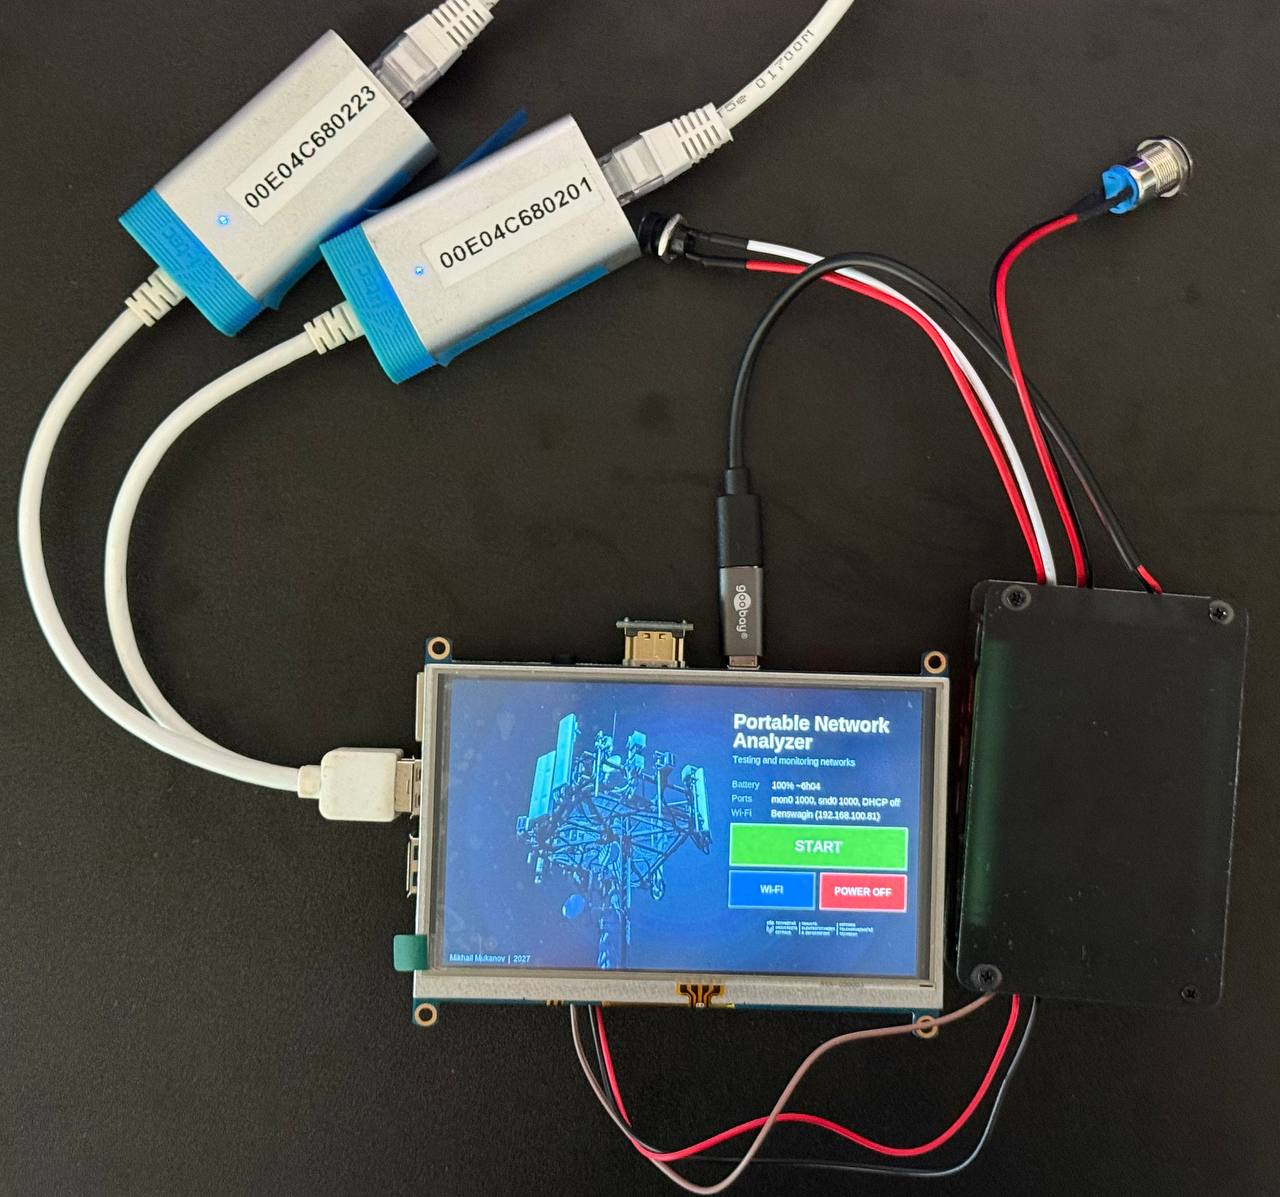
\includegraphics[width=0.75\textwidth]{Figures/device_prototype.jpg}
    \caption[Sestavený prototyp s akumulátorovým modulem]{Sestavený prototyp: Raspberry Pi s displejem, akumulátorový modul, tlačítko napájení a dva označené adaptéry USB/LAN propojené kabelem}
    \label{fig:prototyp}
\end{figure}

\subsection{Napájení z akumulátoru}
\label{sec:napajeni}

Přenosný přístroj musí pracovat bez síťového zdroje, a proto byl doplněn akumulátorovým modulem. Výběr modulu omezila konstrukce displeje. Běžné napájecí nástavby pro Raspberry Pi se k desce připojují zespodu pružnými kontakty na piny GPIO, jenže konektor displeje zabírá piny 1 až 26 z obou stran a nástavbu nebylo kam umístit. Zvolen byl proto samostatný modul Waveshare UPS Module 3S \cite{waveshareups}, který se umisťuje vedle desky. Modul nese tři články typu 18650 zapojené do série, měnič na výstupní napětí 5~V a obvod INA219 pro měření napětí a proudu článků. Osazeny byly články Sony VTC6 s~kapacitou 3000~mAh. Výstup modulu napájí Raspberry Pi přes jeho vlastní konektor micro-USB, takže displej je napájen z desky jako dosud.

Kapacita akumulátoru byla zvolena podle předem naměřené spotřeby přístroje. Spotřeba byla měřena testerem USB zapojeným mezi zdroj a Raspberry Pi, a to v šesti provozních režimech po deseti minutách; výsledky shrnuje Tabulka \ref{tab:spotreba}. Z měření vyplývá, že spotřebu určuje především objem přenášených dat, nikoli složitost prováděné operace. Skenování nástrojem Nmap zvýší odběr oproti nečinnému přístroji jen o 30~mA a pasivní odposlech o 36~mA, kdežto zátěžový test nástrojem iperf3 o 366~mA.

\begin{table}[htbp]
    \caption{Spotřeba přístroje v jednotlivých provozních režimech, měřeno na vstupu 5 V}
    \label{tab:spotreba}
    \centering
    \begin{tabular}{lrr}
        \hline
        Provozní režim & Proud [mA] & Příkon [W] \\
        \hline
        nečinný, podsvícení displeje vypnuto & 678 & 3,40 \\
        nečinný, podsvícení zapnuto & 732 & 3,67 \\
        pasivní odposlech (typický provoz) & 768 & 3,89 \\
        měření propustnosti nástrojem iperf3 & 1098 & 5,52 \\
        skenování nástrojem Nmap & 762 & 3,83 \\
        souběh všech činností (nejhorší případ) & 1242 & 6,10 \\
        \hline
    \end{tabular}
\end{table}

Obvod INA219 je připojen ke sběrnici I2C. Protože piny obvyklé sběrnice zabírá konektor displeje, byla sběrnice vytvořena programově na volných pinech 29 až 31. Stav akumulátoru čte systémová služba každých deset sekund, ze zjištěného napětí určuje zbývající náboj podle vybíjecí křivky naměřené na tomto přístroji a výsledek zapisuje do souboru, z něhož jej řídicí aplikace zobrazuje ve stavovém řádku. Klesne-li napětí článků ve třech po sobě jdoucích měřeních pod 9,6~V, služba přístroj řádně vypne, aby se nepoškodily články ani souborový systém na paměťové kartě. Výsledek vybíjecí zkoušky je uveden v podkapitole \ref{sec:overeni_napajeni}.

\subsection{Programová architektura}
\label{sec:architektura}

Programové vybavení přístroje se skládá z řídicí aplikace, souboru samostatných měřicích skriptů a několika systémových služeb. Vzájemné vazby těchto částí znázorňuje Obrázek \ref{fig:architektura}.

\begin{figure}[htbp]
    \centering
    % Blokove schema programove architektury analyzatoru
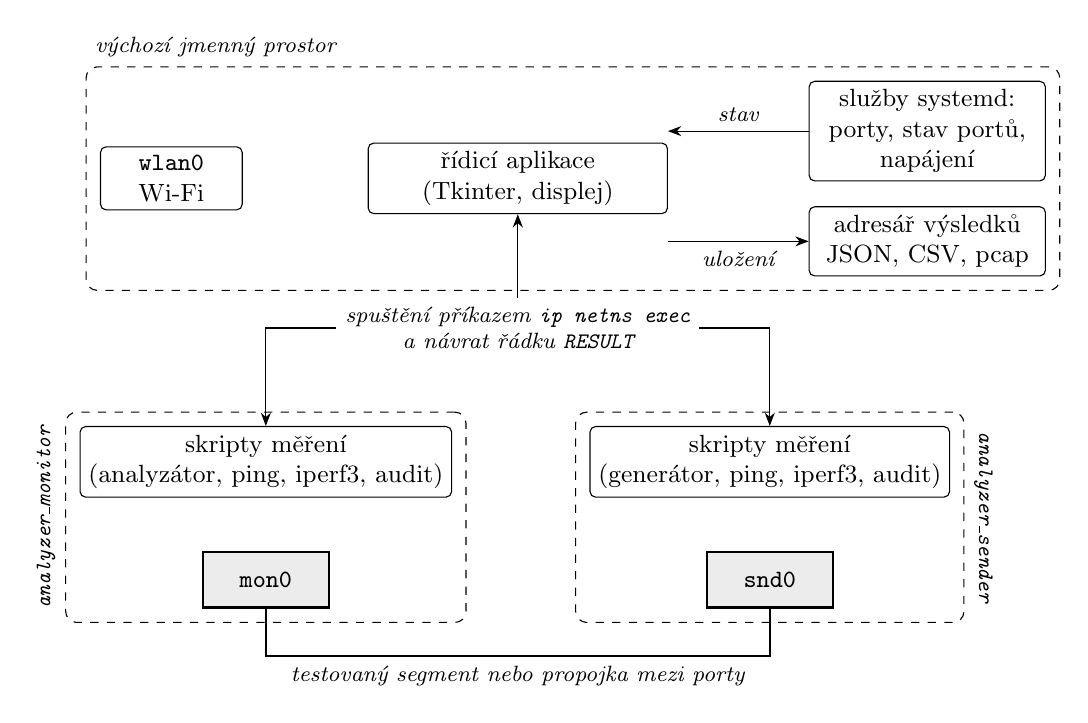
\begin{tikzpicture}[
    font=\small,
    box/.style={draw, rounded corners=2pt, align=center, minimum height=8mm, inner sep=3pt, fill=white},
    port/.style={draw, thick, align=center, minimum width=16mm, minimum height=7mm, fill=gray!15},
    ns/.style={draw, dashed, rounded corners=4pt, inner sep=5pt},
    lbl/.style={font=\footnotesize\itshape, align=center},
    >=Stealth]

    % vychozi jmenny prostor
    \node[box, minimum width=38mm] (gui) at (0,0) {řídicí aplikace\\(Tkinter, displej)};
    \node[box, minimum width=30mm] (sluzby) at (5.2,0.6) {služby systemd:\\porty, stav portů,\\napájení};
    \node[box, minimum width=30mm] (vysledky) at (5.2,-0.8) {adresář výsledků\\JSON, CSV, pcap};
    \node[box, minimum width=18mm] (wlan) at (-4.4,0) {\texttt{wlan0}\\Wi-Fi};
    \node[ns, fit=(gui)(sluzby)(vysledky)(wlan)] (vychozi) {};
    \node[lbl, anchor=south west] at (vychozi.north west) {výchozí jmenný prostor};

    % jmenne prostory testovacich portu
    \node[box, minimum width=40mm] (skripty1) at (-3.2,-3.6) {skripty měření\\(analyzátor, ping, iperf3, audit)};
    \node[port] (mon0) at (-3.2,-5.1) {\texttt{mon0}};
    \node[ns, fit=(skripty1)(mon0)] (nsmon) {};
    \node[lbl, rotate=90, anchor=south] at (nsmon.west) {\texttt{analyzer\_monitor}};

    \node[box, minimum width=40mm] (skripty2) at (3.2,-3.6) {skripty měření\\(generátor, ping, iperf3, audit)};
    \node[port] (snd0) at (3.2,-5.1) {\texttt{snd0}};
    \node[ns, fit=(skripty2)(snd0)] (nssnd) {};
    \node[lbl, rotate=-90, anchor=south] at (nssnd.east) {\texttt{analyzer\_sender}};

    % spusteni skriptu v prostoru portu a navrat vysledku
    \coordinate (rozcesti) at (0,-1.9);
    \draw[<->] (gui.south) -- (rozcesti) -| (skripty1.north);
    \draw[<->] (rozcesti) -| (skripty2.north);
    \node[lbl, fill=white] at (rozcesti) {spuštění příkazem \texttt{ip netns exec}\\a návrat řádku \texttt{RESULT}};
    \draw[->] (sluzby.west) -- node[lbl, above] {stav} (sluzby.west -| gui.east);
    \draw[->] (vysledky.west -| gui.east) -- node[lbl, below] {uložení} (vysledky.west);

    % kabel mezi porty nebo do testovane site
    \draw[thick] (mon0.south) -- ++(0,-0.6) -| node[lbl, pos=0.25, below] {testovaný segment nebo propojka mezi porty} (snd0.south);
\end{tikzpicture}

    \caption{Programová architektura analyzátoru a rozdělení do jmenných prostorů}
    \label{fig:architektura}
\end{figure}

Základem je rozdělení síťových rozhraní do jmenných prostorů popsaných v podkapitole \ref{sec:netns_teorie}. Monitorovací port patří do prostoru \texttt{analyzer\_\allowbreak monitor} s adresami \texttt{10.0.1.10/24} a \texttt{fd00:1::10/64}, port pro generování do prostoru \texttt{analyzer\_\allowbreak sender} s adresami \texttt{10.0.2.10/24} a \texttt{fd00:2::10/64}. Řídicí aplikace zůstává ve výchozím prostoru, kde obsluhuje displej a bezdrátové rozhraní. Mezi oběma prostory neexistuje žádná směrovací cesta, a to ani pro protokol IPv6: jediný provoz, který se z jednoho portu dostane k druhému, je provoz procházející fyzickým kabelem.

Z tohoto uspořádání vyplývá pravidlo, podle něhož je celé programové vybavení členěno. Každá funkce, která potřebuje pracovat v prostoru některého portu, je samostatným skriptem, protože příkaz \texttt{ip netns exec} přesouvá do zvoleného prostoru celý proces a řídicí aplikace musí zůstat ve výchozím prostoru. Skripty jsou použitelné i samostatně z příkazové řádky. Svůj výsledek vypisují na posledním řádku ve tvaru \texttt{RESULT <název skriptu> <JSON>}, který řídicí aplikace přečte a zobrazí. Každý takový výsledek aplikace zároveň uloží do souboru, doplněný o čas s časovým pásmem, o údaj, zda byly hodiny přístroje synchronizovány protokolem NTP, a o kontrolní součet použitého skriptu. Díky tomu je u každého naměřeného čísla dohledatelné, kdy a jakou verzí programu vzniklo.

Jmenné prostory připravuje systémová služba, která se spustí vždy, když se v systému objeví adaptér s odpovídající fyzickou adresou, tedy při startu i při připojení adaptéru za chodu. Služba vytvoří prostor, pokud dosud neexistuje, přesune do něj rozhraní, nastaví adresy a zdvihne linku. Prostor přitom po odpojení adaptéru zůstává zachován, takže se znovu připojený adaptér vrátí do téhož prostoru. Druhá služba sleduje změny stavu linek a adres v obou prostorech a zapisuje je do stavového souboru, z něhož řídicí aplikace čte stav portů bez oprávnění správce.

Přístroj pracuje v takzvaném režimu přístroje. Po zapnutí se bez pracovní plochy operačního systému spustí přímo řídicí aplikace, a to zhruba 36 sekund po startu jádra. Po deseti minutách bez dotyku se obrazovka uzamkne a zhasne, čímž se ušetří 0,35~W; podsvícení displeje je ovládáno pouze mechanickým přepínačem a programově zhasnout nelze.

Zvláštní pozornost byla věnována tomu, co přístroj sám od sebe vysílá do sítě. Přenosný přístroj se může ocitnout v cizí provozní síti a nesmí v ní nic narušit. Po připojení kabelu proto nevysílá nic: jádru bylo zakázáno samočinně hledat směrovač zprávou Router Solicitation, server dnsmasq přidělující adresy se spouští pouze tlačítkem a každý aktivní test se spouští pouze na pokyn obsluhy. Ani po zapnutí serveru dnsmasq se přístroj nevydává za výchozí bránu. Server připojené stanici přiděluje pouze adresu, bez volby výchozí brány a serveru DNS \cite{rfc2132}, a zprávy Router Advertisement nesou nulovou dobu platnosti směrovače, což podle \cite{rfc4861} znamená, že stanice odesílatele nezařadí mezi výchozí směrovače. Důvod se ukázal při připojení notebooku se systémem Windows: ten dává kabelovému rozhraní přednost před bezdrátovým, a kdyby analyzátor ohlásil výchozí bránu, notebook by přes něj posílal veškerý provoz do Internetu, kam přístroj nic nepřeposílá. Takto zůstává notebooku připojení přes Wi-Fi zachováno a s analyzátorem komunikuje pouze v rámci testovaného segmentu.

\section{Realizace generátoru a analyzátoru provozu}
\label{sec:realizace_generatoru}

\subsection{Uživatelské rozhraní}
\label{sec:dotykove_ovladani}

Řídicí aplikace je napsána v jazyce Python s knihovnou Tkinter a pracuje v celoobrazovkovém režimu. Hlavní obrazovka je rozdělena do dvanácti dlaždic, z nichž každá otevírá jednu funkci přístroje (viz Obrázek \ref{fig:gui_home}). Na dlaždici se po provedení testu zobrazuje jeho poslední výsledek, takže obsluha vidí stav přístroje bez otevírání jednotlivých obrazovek. Šedě jsou vyznačeny funkce, které jsou teprve v přípravě.

\begin{figure}[htbp]
    \centering
    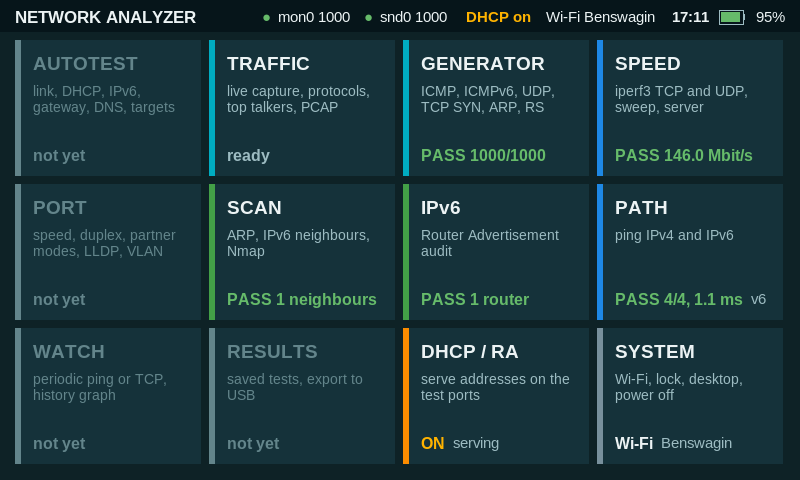
\includegraphics[width=0.72\textwidth]{Figures/gui_home.png}
    \caption{Hlavní obrazovka řídicí aplikace s výsledky posledních testů}
    \label{fig:gui_home}
\end{figure}

Všechny obrazovky funkcí mají shodné uspořádání. Nahoře je stavový řádek s časem, stavem akumulátoru, stavem linky a rychlostí obou portů, stavem serveru DHCP a připojením Wi-Fi. Pod ním je řádek výsledku, který jedním slovem PASS, WARN nebo FAIL a klíčovým číslem shrnuje poslední test, přičemž barva výsledku je vždy doplněna slovem. Dole je řada tlačítek s volbou portu, tlačítky akcí a tlačítkem zpět, vždy na stejném místě.

Rozvržení je podřízeno odporovému dotykovému panelu. Takový panel rozpozná pouze jeden dotyk a jeho přesnost je nejnižší u okrajů činné plochy. Hlavní tlačítka proto měří nejméně 80 na 80 obrazových bodů, což na tomto displeji odpovídá přibližně jedenácti milimetrům, mezi sousedními prvky je mezera nejméně osm bodů a žádný ovládací prvek neleží blíže než patnáct bodů od okraje. Dodržení těchto pravidel na všech obrazovkách ověřuje pomocný skript, který projde všechny obrazovky a změří polohu a velikost každého tlačítka. Aplikace nepoužívá gesta; seznamy se listují tlačítky. Adresy se zadávají přednostně výběrem z nalezených cílů, dále číselnou klávesnicí a teprve v nejnutnějším případě, například při zadávání hesla sítě Wi-Fi, úplnou klávesnicí na obrazovce.

\subsection{Analyzátor provozu}
\label{sec:analyzator}

Pasivní analýzu provozu zajišťuje skript \texttt{sniff\_stats.py}. Samotné zachytávání provádí nástroj tcpdump, který zachycené rámce předává skriptu v binárním formátu pcap. Filtr, kterým obsluha omezí sledovaný provoz, se předává nástroji tcpdump jako výraz jazyka BPF a vyhodnocuje se v jádře \cite{mccanne1993}; rámce, které filtru nevyhovují, se tak k programu vůbec nedostanou. Skript z každého rámce rozebere hlavičky Ethernet, případně značku VLAN, IPv4 nebo IPv6 včetně řetězce rozšiřujících hlaviček, a dále TCP, UDP, ICMP, ICMPv6 nebo ARP. Pro rozbor nebyla použita knihovna Scapy, protože je na procesoru použité desky pro souvislý proud rámců příliš pomalá.

Jednou za sekundu skript vypíše řádek se souhrnnými ukazateli. Jde o počet rámců a bitů za sekundu, průměrnou velikost rámce, podíl jednotlivých protokolů, poměr provozu IPv4 a IPv6, počet různých stanic a pět stanic s největším objemem odeslaných dat. Tyto ukazatele odpovídají statistikám, které nabízí analyzátor Wireshark \cite{wiresharkstat}. Řádek obsahuje také několik posledních zachycených rámců i s jejich rozborem, takže řídicí aplikace nedostává jednu zprávu za každý rámec, ale jednu souhrnnou zprávu za sekundu. Na konci zachytávání skript uvede, kolik rámců jádro nestihlo předat a zahodilo, takže případná ztráta při zachytávání je změřena, nikoli odhadnuta.

Při ověřování se ukázalo, že na rozhraních jsou ve výchozím stavu zapnuty funkce, jimiž síťová karta a jádro slučují po sobě jdoucí segmenty TCP do jednoho velkého paketu. Analyzátor pak místo rámců o velikosti nejvýše 1514~bajtů viděl pakety o velikosti desítek kilobajtů a počty i průměrná velikost byly zkreslené. Skript proto tyto funkce po dobu zachytávání na sledovaném portu vypíná a po skončení je vrací do původního stavu.

Nad skriptem je postavena obrazovka TRAFFIC (viz Obrázek \ref{fig:gui_traffic}). V horní části ukazuje hlavní ukazatele, pod nimi pruh s podílem protokolů, vlevo nejaktivnější stanice a vpravo průběžný výpis posledních rámců. Tlačítko PAUSE výpis zastaví, zatímco počítání pokračuje, a zobrazí posledních dvě stě rámců po stránkách. Dotykem na rámec se otevře jeho rozbor po jednotlivých vrstvách; Obrázek \ref{fig:gui_packet_ra} ukazuje rozbor zprávy Router Advertisement včetně příznaků a nesených voleb. Tlačítko FILTER nabízí předvolby TCP, UDP, ICMP, ARP, DHCP, ND/RA a DNS a filtr podle zvolené stanice; zvolená předvolba se převede na výraz BPF a zachytávání se s ním spustí znovu. Tlačítko SAVE uloží zachycený provoz ve formátu pcap pro rozbor v analyzátoru Wireshark, průběh ukazatelů ve formátu CSV a souhrnný výsledek ve formátu JSON.

\begin{figure}[htbp]
    \centering
    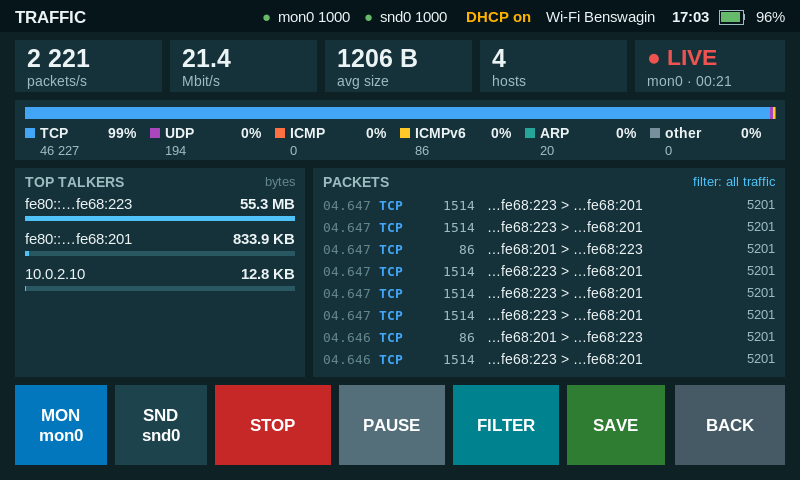
\includegraphics[width=0.72\textwidth]{Figures/gui_traffic.png}
    \caption{Obrazovka TRAFFIC při zachytávání provozu na monitorovacím portu}
    \label{fig:gui_traffic}
\end{figure}

\begin{figure}[htbp]
    \centering
    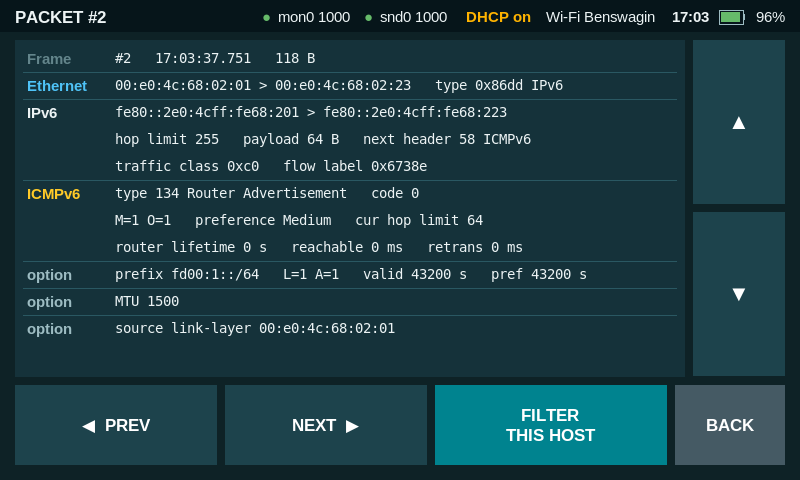
\includegraphics[width=0.72\textwidth]{Figures/gui_packet_ra.png}
    \caption{Rozbor zachycené zprávy Router Advertisement po jednotlivých vrstvách}
    \label{fig:gui_packet_ra}
\end{figure}

\subsection{Generátor paketů}
\label{sec:generator}

Nástroj iperf3 měří propustnost, ale neumožňuje odeslat přesně zvolený počet paketů určitého typu. K tomu slouží skript \texttt{pkt\_gen.py}. Umí sestavit zprávy ICMP a ICMPv6 Echo Request, datagramy UDP, segmenty TCP s příznakem SYN, dotazy ARP a zprávy Router Solicitation, a to v zadaném počtu, rychlosti a velikosti rámce. Rámce sestaví předem knihovnou Scapy \cite{carter2024} a odesílá je přímo na linkovou vrstvu, takže pomalá knihovna v odesílací smyčce vůbec nefiguruje a rychlost je omezena jen procesorem a sběrnicí. Cílem smí být pouze adresy testovacího stanoviště; na jiné adresy skript bez výslovného potvrzení nic neodešle.

Obrazovka GENERATOR spojuje generátor s analyzátorem (viz Obrázek \ref{fig:gui_generator}). Pakety odesílá jeden port přístroje a druhý port je ve vlastním jmenném prostoru počítá analyzátorem s filtrem na fyzickou adresu odesílatele a zvolený typ paketu. Pakety tak prokazatelně projdou kabelem z jednoho jmenného prostoru do druhého a výsledek je okamžitě porovnán: shodný počet odeslaných a přijatých paketů znamená výsledek PASS, rozdíl je vykázán jako ztráta.

\begin{figure}[htbp]
    \centering
    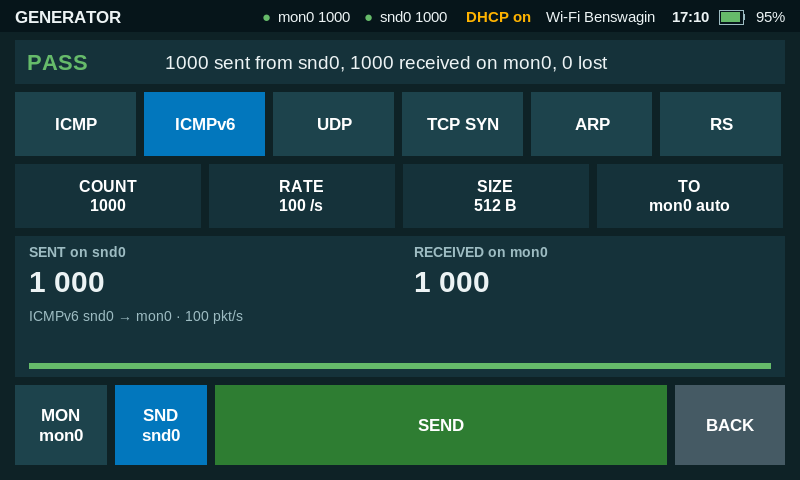
\includegraphics[width=0.72\textwidth]{Figures/gui_generator.png}
    \caption[Generátor paketů: odesláno portem \texttt{snd0}, spočítáno na \texttt{mon0}]{Generátor paketů: tisíc zpráv ICMPv6 odeslaných portem \texttt{snd0} a spočítaných na portu \texttt{mon0}}
    \label{fig:gui_generator}
\end{figure}

\subsection{Měření zpoždění, propustnosti a ztrátovosti}
\label{sec:mereni_realizace}

Zpoždění a dostupnost protistrany měří obrazovka PATH testem ping. Propustnost, ztrátovost a rozptyl zpoždění měří obrazovka SPEED nástrojem iperf3. Oba testy potřebují znát cíl. V první verzi aplikace byly adresy cílů zapsány napevno a později je bylo možné vyhledat tlačítkem popsaným v podkapitole \ref{sec:vyhledavani_sousedu}. Nyní si cíl, není-li zadán, vyhledají testy samy, a to v tomto pořadí: adresa, kterou připojené stanici přidělil server DHCP přístroje, dále sousedé známí jádru a nakonec odpověď na zprávu Echo Request zaslanou na skupinovou adresu všech uzlů. Každý kandidát je před použitím ověřen novým dotazem ARP nebo Neighbor Solicitation, protože záznam o přidělené adrese přetrvává ještě hodiny po odpojení stanice. Pozná-li přístroj podle fyzické adresy, že odpověděl jeho vlastní druhý port, oznámí, že porty jsou propojeny mezi sebou.

Nenajde-li test cíl nebo cíl neodpoví, uvede obsluze důvod a doporučení. Na propojce mezi porty tak například test protokolem IPv4 vysvětlí, že porty patří do různých podsítí a nic mezi nimi nesměruje, a doporučí použít protokol IPv6 (viz Obrázek \ref{fig:gui_path_loop}). Odpoví-li stanice na dotaz ARP nebo Neighbor Solicitation, ale ne na ping, přístroj ohlásí, že stanice je připojena, ale ping blokuje její firewall.

\begin{figure}[htbp]
    \centering
    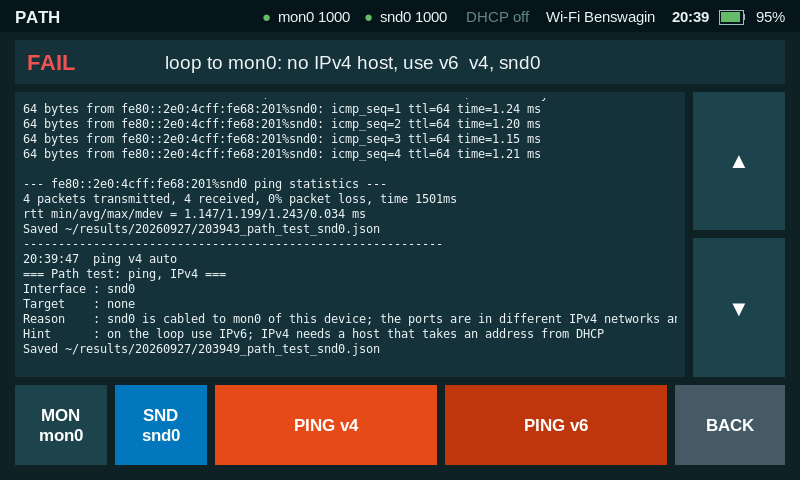
\includegraphics[width=0.72\textwidth]{Figures/gui_path_loop.png}
    \caption[Test ping na propojce mezi porty s vysvětlením chybějícího cíle]{Test ping na propojce mezi porty: cíl IPv6 nalezen samočinně, u IPv4 přístroj vysvětluje, proč cíl neexistuje}
    \label{fig:gui_path_loop}
\end{figure}

Zátěžové testy řídí skript \texttt{perf\_test.py}, který spouští nástroj iperf3 \cite{iperf3} s výstupem ve formátu JSON a čísla přebírá z něj, nikoli z textového výpisu. Obsluha volí protokol TCP nebo UDP, verzi protokolu IP, u protokolu UDP vysílací rychlost, dobu testu a směr, tedy zda data odesílá analyzátor, nebo protistrana. U protokolu UDP přístroj vedle propustnosti zobrazí počet ztracených datagramů a rozptyl zpoždění (viz Obrázek \ref{fig:gui_speed_udp}). Ke každému výsledku skript zaznamená průměrné vytížení procesoru, teplotu čipu na začátku a na konci testu a údaj, zda procesor nebyl kvůli teplotě nebo napájení přibržděn. Měření s přibržděným procesorem je označeno varováním, protože jeho výsledek nelze porovnávat s ostatními.

\begin{figure}[htbp]
    \centering
    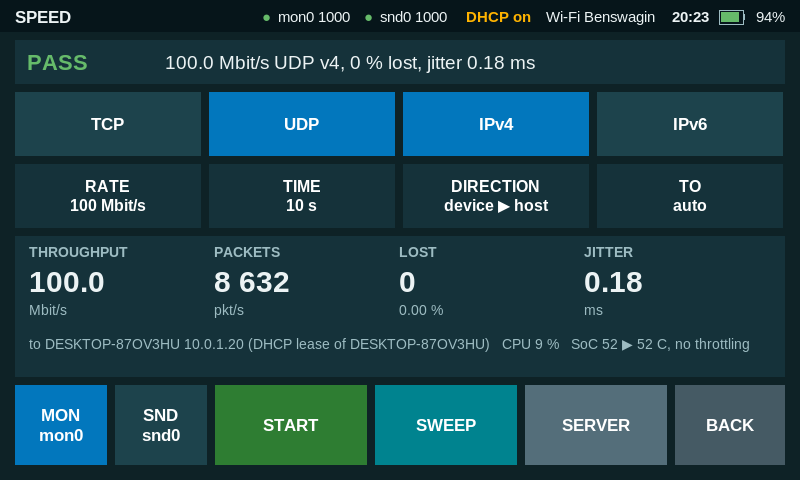
\includegraphics[width=0.72\textwidth]{Figures/gui_speed_udp.png}
    \caption[Měření protokolem UDP proti notebooku]{Měření protokolem UDP proti notebooku: propustnost, počet datagramů za sekundu, ztráta a rozptyl zpoždění}
    \label{fig:gui_speed_udp}
\end{figure}

Obrazovka SPEED nabízí ještě dvě další funkce. Tlačítko SWEEP spustí měření protokolem UDP postupně pro sedm velikostí rámce, které pro Ethernet doporučuje \cite{rfc2544}, a výsledky zobrazí v tabulce. Velikost rámce se přepočítává na velikost dat datagramu zvlášť pro protokol IPv4 a IPv6, protože hlavička IPv6 je o dvacet bajtů delší. Rámec o velikosti 64~bajtů pro IPv6 sestavit nelze: hlavičky Ethernet, IPv6 a UDP spolu s kontrolním součtem rámce mají samy 66~bajtů a nástroj iperf3 potřebuje alespoň 16~bajtů dat. Řada pro IPv6 proto začíná rámcem o velikosti 82~bajtů, což \cite{rfc5180} u měřicích nástrojů připouští. Tlačítko SERVER naopak spustí na zvoleném portu server iperf3 a na displeji ukáže adresy, na které se má připojit protistrana; měří tedy notebook proti analyzátoru. Protože metody podle \cite{rfc2544} nepatří do provozních sítí \cite{rfc6815}, spustí přístroj měření proti adrese mimo testovací stanoviště teprve po opakovaném potvrzení a rozmítání velikostí rámce mimo stanoviště nespustí vůbec. Je-li cílem druhý port téhož přístroje, spustí skript na něm po dobu testu server iperf3 sám, takže měření na propojce mezi porty nevyžaduje žádnou přípravu.

\subsection{Adresní autokonfigurace protokolu IPv6}
\label{sec:autokonfigurace}

Požadavek na plnou podporu protokolu IPv6 se při realizaci ukázal jako nejnáročnější část konfigurace, a to kvůli odlišné povaze obou protokolů. Zatímco stanice s protokolem IPv4 nemá bez klienta DHCP jak adresu získat, protokol IPv6 nabízí vedle stavového serveru DHCPv6 také bezstavovou autokonfiguraci, při níž si stanice sestaví adresu sama z prefixu inzerovaného ve zprávě Router Advertisement. Kterou cestu stanice zvolí, určuje samotná zpráva: příznak M ji odkazuje na server DHCPv6, zatímco příznak A, nesený u každého prefixu zvlášť, teprve povoluje sestavení adresy z tohoto prefixu \cite{nastase2024}.

Server dnsmasq běží v každém jmenném prostoru zvlášť a obsluhuje pouze rozhraní svého prostoru. V první realizaci byl rozsah adres pro protokol IPv6 zapsán jako jediná konkrétní adresa, tedy \texttt{-{}-dhcp-range=\allowbreak fd00:1::20,\allowbreak fd00:1::20,\allowbreak 64,\allowbreak 12h}. Toto zdánlivě neškodné zúžení rozsahu vedlo k tomu, že server nastavil příznaky ve zprávě Router Advertisement způsobem uvedeným v Tabulce \ref{tab:ra_flags}. Hodnoty byly odečteny na cílové stanici nástrojem \texttt{rdisc6}, který zprávu vyžádá a vypíše její obsah.

\begin{table}[htbp]
    \caption{Příznaky ve zprávě Router Advertisement před úpravou a po ní}
    \label{tab:ra_flags}
    \centering
    \begin{tabular}{lcc}
        \hline
        Příznak & Původní konfigurace & Po doplnění \texttt{slaac} \\
        \hline
        M -- Stateful address configuration & Yes & Yes \\
        O -- Stateful other configuration & Yes & Yes \\
        A -- Autonomous address configuration & No & Yes \\
        On-link & Yes & Yes \\
        \hline
    \end{tabular}
\end{table}

Autokonfiguraci tedy bránily dvě okolnosti současně. Nastavený příznak M odkazoval stanici na server DHCPv6 a zhasnutý příznak A u prefixu zakazoval sestavit z něj adresu vlastními silami. Server dnsmasq nastavuje obojí právě tímto způsobem, je-li rozsah zadán konkrétní adresou, neboť takový zápis chápe jako pokyn k výhradně stavovému přidělování. Řešením se ukázalo doplnění klíčového slova \texttt{slaac} do téhož parametru, tedy \texttt{-{}-dhcp-range=\allowbreak fd00:1::20,\allowbreak fd00:1::20,\allowbreak slaac,\allowbreak 64,\allowbreak 12h}. Po této jediné úpravě začal analyzátor inzerovat prefix se zdviženým příznakem A, aniž by přestal obsluhovat stavové požadavky.

Účinek úpravy se projevil okamžitě. Jádro cílové stanice sestavilo z inzerovaného prefixu adresu \texttt{fd00:1::\allowbreak 2e0:\allowbreak 4cff:\allowbreak fe68:\allowbreak 216} označenou v systémovém výpisu příznakem \texttt{proto kernel\_ra}, tedy adresu vytvořenou přímo jádrem bez účasti jakéhokoli procesu v uživatelském prostoru. Identifikátor rozhraní v její druhé polovině odpovídá fyzické adrese cílového rozhraní \texttt{00:\allowbreak e0:\allowbreak 4c:\allowbreak 68:\allowbreak 02:\allowbreak 16} převedené postupem EUI-64, takže adresa protistrany je z fyzické adresy vypočitatelná.

Z pozorování plyne závěr podstatnější než samotná oprava konfigurace. Rozdíl mezi protokoly nespočívá v množství ruční práce, neboť moderní správci síťových připojení si profil vytvoří samočinně u obou protokolů. Rozdíl spočívá v tom, zda je na cílové stanici vůbec zapotřebí nějaký proces: u protokolu IPv4 bez klienta DHCP adresa nevznikne nikdy, kdežto u protokolu IPv6 přidělí jádro adresu lokální linky ihned po zdvižení rozhraní a při zdviženém příznaku A sestaví z inzerovaného prefixu i adresu širšího dosahu.

\subsection{Audit zpráv Router Advertisement}
\label{sec:audit_ra}

Zjištění z předchozí podkapitoly ukázala, že o způsobu adresování celého segmentu rozhoduje obsah jediné zprávy. Stanice si sama neověřuje, kdo zprávu Router Advertisement odeslal, a přijme ji od kohokoli, kdo ji v segmentu vyšle \cite{rfc4861}. Pro diagnostický přístroj z toho plyne úkol umět tuto zprávu zachytit, rozebrat a posoudit, zda odpovídá požadavkům normy. Tento úkol plní skript \texttt{ra\_audit.py}, který obsluha spouští z obrazovky IPv6.

Skript nejprve spustí naslouchání zprávám ICMPv6 a poté sám vyšle zprávu Router Solicitation na skupinovou adresu \texttt{ff02::2}, takže na odpověď nemusí čekat po dobu periodického ohlašování. Ze zachycených zpráv vyčte hodnotu Cur Hop Limit, příznaky M a O, preferenci a dobu platnosti směrovače, z nesených voleb pak inzerované prefixy s jejich příznaky a dobami životnosti, hodnotu MTU, adresy serverů DNS a fyzickou adresu odesílatele. Nad rozebranou zprávou provede soubor kontrol: zda hodnota Hop Limit v hlavičce odpovídá předepsaným 255 a zda je zdrojová adresa adresou lokální linky \cite{rfc4861}, zda má prefix se zdviženým příznakem A délku 64~bitů \cite{rfc4862}, zda preferovaná doba životnosti nepřevyšuje dobu platnosti, zda hodnota MTU neklesá pod minimum 1280~bajtů \cite{rfc8200} a zda se fyzická adresa v rámci shoduje s adresou uvedenou ve volbě. Každé hlášení nese odkaz na příslušný dokument přímo v textu.

Při ověřování se ukázalo, že rozdělení zpráv pouze na vlastní a cizí podle fyzické adresy odesílatele nestačí, neboť zachytávací rozhraní vidí i rámce odcházející z téhož portu. Přístroj tak ohlašoval přítomnost směrovače ve chvíli, kdy pozoroval vysílání vlastního serveru dnsmasq. Původ zprávy je proto rozlišován ve třech stupních: rámec odeslaný týmž portem, rámec z druhého portu téhož přístroje zachycený po vedení a rámec cizího směrovače, který jediný je důvodem k výstraze.

Z téhož mechanismu plyne omezení: přístroj nedokáže vyžádat zprávu Router Advertisement od serveru běžícího na tomtéž portu, protože žádost odchází přímo na linkové vrstvě mimo síťový zásobník a server ji nezaznamená. Zpráva musí projít po vedení, a audit se proto ověřuje v uspořádání, kdy jsou oba porty propojeny jediným kabelem; každý z nich pak slyší ohlašování protějšku.

\subsection{Vyhledávání sousedů}
\label{sec:vyhledavani_sousedu}

Adresy protistrany zapsané napevno platí na laboratorním stanovišti, nikoli však v terénu, kde připojené zařízení může mít adresní plán zcela vlastní. Zjištění, že adresa sestavená bezstavovou autokonfigurací je z fyzické adresy vypočitatelná, nabízí cestu, jak tento předpoklad odstranit. Tuto funkci zajišťuje skript \texttt{neigh\_scan.py}, spouštěný tlačítkem NEIGHBORS z obrazovky SCAN.

Skript vyšle zprávu Echo Request na skupinovou adresu všech uzlů \texttt{ff02::1} a odpovědi doplní o obsah tabulky sousedů udržované jádrem. Ke každé nalezené fyzické adrese dopočte postupem EUI-64 identifikátor rozhraní a porovná jej s adresou lokální linky, kterou soused skutečně používá. Shoda znamená, že stanice sestavuje identifikátor klasicky z fyzické adresy; neshoda, že používá identifikátor neprozrazující hardware podle \cite{rfc7217}, jehož smyslem je zabránit sledování stanice napříč sítěmi. Je-li odvození možné, sestaví skript pro každý prefix nastavený na portu kandidáta na adresu a ověří jej testem dostupnosti, takže do výsledku vstupuje potvrzená adresa, nikoli domněnka. Týmž tlačítkem se spouští i skenování protokolem ARP v rozsahu adres portu, takže obsluha vidí výsledek obou protokolů vedle sebe.

\section{Zhodnocení dosažených výsledků}
\label{sec:zhodnoceni}

Prototyp byl ověřován ve třech uspořádáních. Na počátku byl prototyp ověřen v laboratoři počítačových sítí, kde byl propojen dvěma kabely s cílovou stanicí se systémem Linux (viz Obrázek \ref{fig:zapojeni}); stejné uspořádání s osobním počítačem se systémem Linux posloužilo později i k měření autokonfigurace. Většina dalších měření proběhla v uspořádání, kdy jsou oba porty přístroje propojeny jediným kabelem mezi sebou. Takové měření je opakovatelné a nevyžaduje žádné další zařízení, přístroj však v něm měří sám sebe. Proto byly výsledky ověřeny ještě s notebookem se systémem Windows 11, k němuž byly oba porty připojeny přes dva další adaptéry USB/LAN. Toto třetí uspořádání odhalilo několik skutečností, které propojka mezi porty skrývá; jsou popsány v podkapitole \ref{sec:overeni_notebook}.

\begin{figure}[htbp]
    \centering
    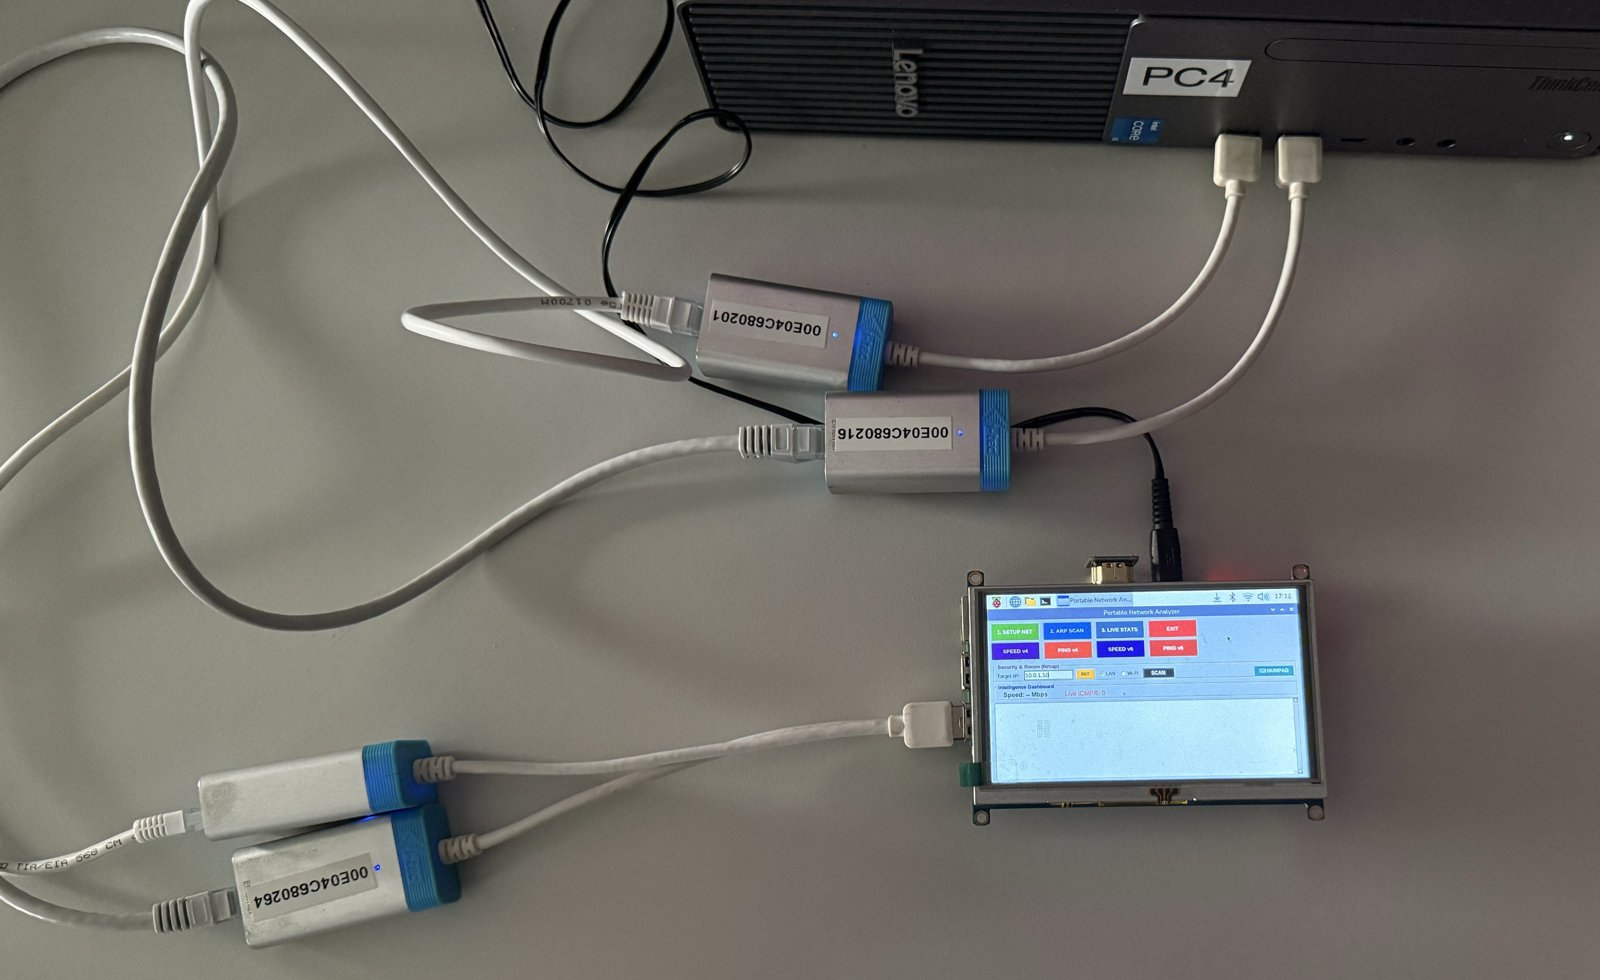
\includegraphics[width=0.75\textwidth]{Figures/lab_connection.jpg}
    \caption{Fyzické zapojení analyzátoru a cílové stanice v laboratoři}
    \label{fig:zapojeni}
\end{figure}

\subsection{Ověření automatické konfigurace adres}
\label{sec:overeni_autokonfigurace}

Chování adresní autokonfigurace popsané v podkapitole \ref{sec:autokonfigurace} bylo ověřeno měřením, při němž byl analyzátor propojen s cílovou stanicí oběma porty současně. Monitorovací port byl restartován s doplněným klíčovým slovem \texttt{slaac}, zatímco port pro generování provozu zůstal v původním nastavení jako kontrolní vzorek. Adresy přidělené oběma rozhraním cílové stanice shrnuje Tabulka \ref{tab:adresy}.

\begin{table}[htbp]
    \caption{Adresy přidělené cílové stanici na obou testovacích portech}
    \label{tab:adresy}
    \centering
    \begin{tabular}{lll}
        \hline
        Port analyzátoru & Adresa cílové stanice & Způsob získání \\
        \hline
        monitorovací, A = 1 & \texttt{10.0.1.20} & DHCPv4 \\
        monitorovací, A = 1 & \texttt{fd00:1::20/128} & stavově, DHCPv6 \\
        monitorovací, A = 1 & \texttt{fd00:1::2e0:4cff:fe68:216/64} & bezstavově, jádrem ze zprávy RA \\
        generující, A = 0 & \texttt{10.0.2.20} & DHCPv4 \\
        generující, A = 0 & \texttt{fd00:2::20/128} & stavově, DHCPv6 \\
        \hline
    \end{tabular}
\end{table}

Podstatou měření je rozdíl mezi oběma řádky s protokolem IPv6. Na monitorovacím portu vznikla vedle stavově přidělené adresy také adresa sestavená jádrem z inzerovaného prefixu, kdežto na kontrolním portu se zhasnutým příznakem A žádná taková adresa nevznikla, přestože obě rozhraní byla po celou dobu aktivní a obsluhována týmž zařízením. Doplnění jediného klíčového slova je tedy skutečnou a jedinou příčinou pozorované změny. Testy dostupnosti na adresy přidělené stavově i na adresu sestavenou bezstavově proběhly bez ztráty paketů s dobou odezvy okolo jedné milisekundy.

\subsection{Ověření auditu protokolu IPv6}
\label{sec:overeni_auditu}

Audit byl ověřen na propojce mezi porty, kde se obě linky ustavily na rychlosti 1000~Mbit/s v plně duplexním režimu. Rozbor zprávy zachycené na portu \texttt{snd0} po zapnutí serveru dnsmasq zachycuje Obrázek \ref{fig:gui_ra_audit}. Přístroj správně určil, že ohlašujícím směrovačem je jeho vlastní druhý port, neboť fyzická adresa odesílatele odpovídá jednomu z jeho rozhraní a zpráva byla přijata po vedení. Z obsahu zprávy vyčetl prefix \texttt{fd00:1::/64} s příznaky L a A, dobu platnosti 43\,200 sekund a hodnotu MTU 1500~bajtů. Nulovou dobu platnosti směrovače, zavedenou záměrně podle podkapitoly \ref{sec:architektura}, vyhodnotil pouze jako informaci, protože zpráva pochází z vlastního přístroje. Upozornil také, že zpráva současně nese příznak M i prefix s příznakem A, tedy nabízí stanicím stavový i bezstavový zdroj adresy; jde o přesný popis chování serveru dnsmasq po doplnění klíčového slova \texttt{slaac}, nikoli o chybu, a odpovídá to i Tabulce \ref{tab:adresy}.

\begin{figure}[htbp]
    \centering
    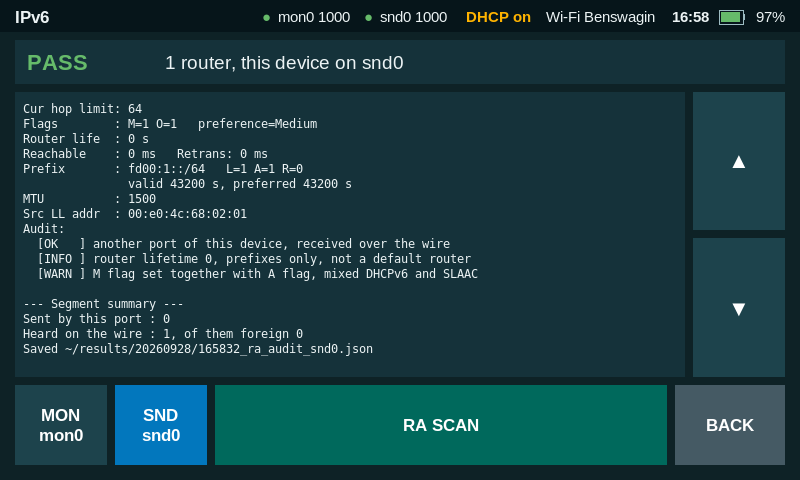
\includegraphics[width=0.72\textwidth]{Figures/gui_ra_audit.png}
    \caption{Audit zprávy Router Advertisement přijaté od druhého portu přístroje}
    \label{fig:gui_ra_audit}
\end{figure}

Týmž uspořádáním bylo možné potvrdit i Tabulku \ref{tab:ra_flags} měřením provedeným samotným přístrojem: s původní konfigurací ohlásil audit u prefixu zhasnutý příznak A a upozornění, že bezstavová autokonfigurace je zakázána, po doplnění klíčového slova \texttt{slaac} příznak zdvižený. Samotné kontroly nešlo ověřit na skutečném provozu, protože v testovaném segmentu žádný nesprávně nastavený směrovač není. Byly proto ověřeny na programově sestaveném pracovišti ze dvou dočasných jmenných prostorů spojených virtuálním párem rozhraní, do něhož byla vložena záměrně vadná zpráva s hodnotou Hop Limit 64, zdrojovou adresou mimo lokální linku, prefixem délky 48~bitů se zdviženým příznakem A, preferovanou dobou životnosti vyšší než dobou platnosti, hodnotou MTU 1200~bajtů a odlišnou fyzickou adresou ve volbě. Přístroj označil všechny nesrovnalosti současně a zprávu vyhodnotil jako zprávu cizího směrovače.

Vyhledání sousedů bylo ověřeno na téže propojce (viz Obrázek \ref{fig:gui_neighbours}). Přístroj nalezl jediného souseda, dopočetl z jeho fyzické adresy identifikátor rozhraní, zjistil shodu s adresou lokální linky a pro oba prefixy na portu sestavil adresu, kterou ověřil jako dosažitelnou. Nejzřetelnější je však srovnání obou protokolů v témže okamžiku, které shrnuje Tabulka \ref{tab:sousede}. Skenování protokolem ARP nenalezlo nikoho, protože porty patří do různých podsítí a na protějším konci neběží žádný klient DHCP. Protokol IPv6 nalezl na témže vedení téhož souseda a jeho adresu ověřil, a to bez jediného procesu zajišťujícího konfiguraci. Tvrzení z podkapitoly \ref{sec:autokonfigurace} je tak podloženo měřením.

\begin{figure}[htbp]
    \centering
    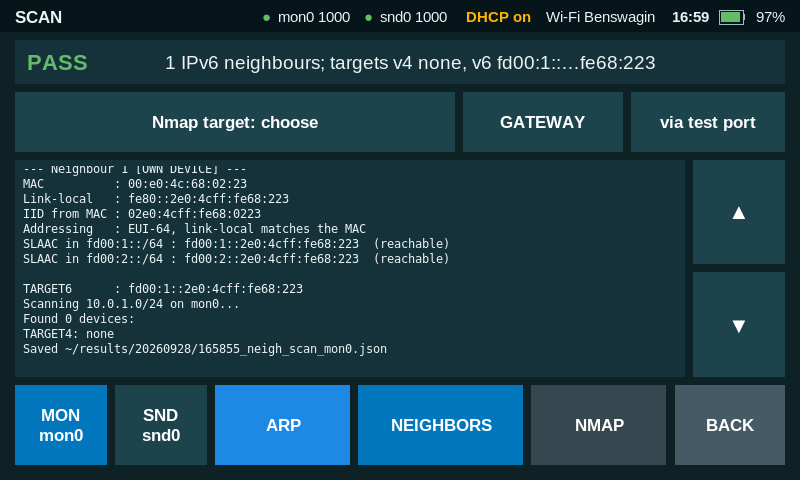
\includegraphics[width=0.72\textwidth]{Figures/gui_neighbours.png}
    \caption[Vyhledání sousedů protokolem IPv6 a skenování ARP]{Vyhledání sousedů: adresy odvozené postupem EUI-64 a ověřené testem dostupnosti, skenování ARP bez výsledku}
    \label{fig:gui_neighbours}
\end{figure}

\begin{table}[htbp]
    \caption{Vyhledání protistrany na témže vedení oběma protokoly}
    \label{tab:sousede}
    \centering
    \begin{tabular}{lll}
        \hline
        Protokol & Použitý postup & Výsledek \\
        \hline
        IPv4 & skenování ARP v rozsahu \texttt{10.0.1.0/24} & nenalezena žádná stanice \\
        IPv6 & dotaz na \texttt{ff02::1} a tabulka sousedů & nalezen soused, adresa ověřena \\
        \hline
    \end{tabular}
\end{table}

\subsection{Přesnost a meze analyzátoru}
\label{sec:overeni_analyzatoru}

Přesnost analyzátoru byla ověřena na propojce mezi porty tak, že tentýž proces, který počítal statistiku, zároveň ukládal zachycený provoz do souboru, a ten byl poté nezávisle přepočítán nástrojem tcpdump s filtry pro jednotlivé protokoly a nástrojem capinfos. Při smíšeném provozu složeném ze sta testů ping protokolem IPv4, sta testů protokolem IPv6 a pětisekundového přenosu TCP se všechny počty shodovaly přesně (viz Tabulka \ref{tab:presnost}). Při přenosu UDP rychlostí 10~Mbit/s po dobu třiceti sekund napočítal analyzátor 37\,503 datagramů, zatímco iperf3 odeslal 37\,501 datagramů bez ztráty; rozdíl dvou datagramů odpovídá dvěma řídicím zprávám, které si iperf3 vyměňuje při zahájení testu. Rozbor jednotlivých rámců zobrazovaný na obrazovce TRAFFIC byl navíc porovnán s nástrojem tshark, tedy s rozborem analyzátoru Wireshark: na 58 rámcích všech podporovaných typů se shodovalo všech 781 porovnaných položek.

\begin{table}[htbp]
    \caption{Počty rámců podle protokolů: analyzátor přístroje a nezávislý přepočet uloženého souboru}
    \label{tab:presnost}
    \centering
    \begin{tabular}{lrr}
        \hline
        Protokol & Analyzátor přístroje & Přepočet nástrojem tcpdump \\
        \hline
        TCP & 11\,251 & 11\,251 \\
        UDP & 0 & 0 \\
        ICMP & 200 & 200 \\
        ICMPv6 & 202 & 202 \\
        ARP & 4 & 4 \\
        celkem & 11\,657 & 11\,657 \\
        \hline
    \end{tabular}
\end{table}

Mez analyzátoru byla hledána postupným zvyšováním rychlosti přenosu UDP. Vyjádřit ji v megabitech za sekundu nelze, protože rozhoduje počet rámců: zpracování každého rámce stojí stejnou práci bez ohledu na jeho velikost. S krátkými rámci o velikosti 162~bajtů zachytil analyzátor bez ztráty 22\,498 rámců za sekundu; při 26\,247 rámcích za sekundu už ztratil 11,8~\% a výše se ustálil zhruba na 23\,000 rámcích za sekundu. Úzkým místem je jedno jádro procesoru, na němž běží rozbor hlaviček a které bylo vytíženo z 99~\%, zatímco ostatní jádra měla rezervu. U rámců plné délky 1514~bajtů odpovídá tato mez přibližně 270~Mbit/s, tedy zhruba stropu sběrnice USB 2.0, takže dlouhé rámce analyzátor stíhá, krátké při vysoké rychlosti nikoli.

Účinek filtru vyhodnocovaného v jádře byl změřen při přenosu TCP rychlostí 50~Mbit/s, k němuž byly přidány zprávy ICMPv6. Bez filtru zatěžoval rozbor procesor z 27,2~\%, s filtrem \texttt{icmp6} jen z 0,4~\% a statistika obsahovala pouze zprávy ICMPv6. Rámce, které filtru nevyhověly, se tedy k programu vůbec nedostaly.

\subsection{Výkon generátoru paketů}
\label{sec:overeni_generatoru}

Generátor odeslal tisíc zpráv ICMPv6 Echo Request rychlostí sto zpráv za sekundu z portu \texttt{snd0} a analyzátor jich na portu \texttt{mon0} napočítal přesně tisíc (viz Obrázek \ref{fig:gui_generator}); stejný výsledek dalo všech šest podporovaných typů paketů i opačný směr. Nejvyšší rychlost byla měřena bez zachytávání, podle čítače přijatých rámců adaptéru. S rámci o velikosti 100~bajtů dosáhl generátor 83\,764 rámců za sekundu při vytížení jednoho jádra z 97~\%, s rámci o velikosti 1514~bajtů přenesl 157~Mbit/s při vytížení 17~\% a ve všech případech bez ztráty na přijímající straně. Krátké rámce tedy omezuje procesor, dlouhé sběrnice. Smyslem generátoru přitom není co nejvyšší rychlost; nástroj iperf3 s~krátkými datagramy vyšle rámců za sekundu více, jak ukazuje podkapitola \ref{sec:mereni_propustnosti}. Generátor slouží k odeslání přesně zvoleného počtu paketů určitého typu a k ověření, že všechny dorazily.

\subsection{Měření propustnosti}
\label{sec:mereni_propustnosti}

Propustnost protokolem TCP byla měřena proti notebooku z obou portů a oběma verzemi protokolu IP. Výsledky shrnuje Tabulka \ref{tab:propustnost} a jeden z nich zachycuje Obrázek \ref{fig:gui_speed_tcp}. Všechna čtyři měření se pohybují mezi 273 a 276~Mbit/s a shodují se s měřením provedeným dříve v laboratoři, kdy vyšlo 276~Mbit/s pro IPv4 a 274~Mbit/s pro IPv6. Rozdíl mezi protokoly je v jednotkách megabitů a odpovídá delší hlavičce IPv6 rozebrané v podkapitole \ref{sec:ipv4_ipv6}.

\begin{table}[htbp]
    \caption{Propustnost protokolem TCP, test v délce deseti sekund}
    \label{tab:propustnost}
    \centering
    \begin{tabular}{llr}
        \hline
        Uspořádání & Protokol & Propustnost [Mbit/s] \\
        \hline
        port \texttt{mon0} proti notebooku & IPv4 & 274,0 \\
        port \texttt{mon0} proti notebooku & IPv6 & 274,2 \\
        port \texttt{snd0} proti notebooku & IPv4 & 273,3 \\
        port \texttt{snd0} proti notebooku & IPv6 & 275,0 \\
        propojka mezi porty & IPv6 & 150,5 \\
        \hline
    \end{tabular}
\end{table}

\begin{figure}[htbp]
    \centering
    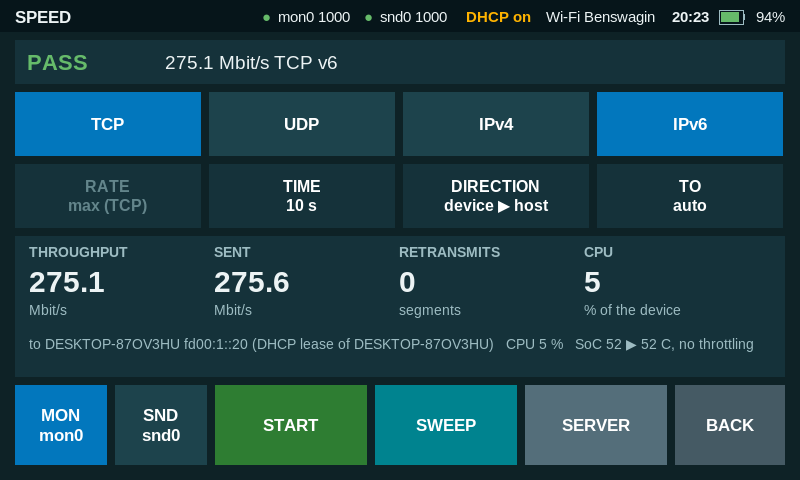
\includegraphics[width=0.72\textwidth]{Figures/gui_speed_tcp.png}
    \caption{Měření propustnosti protokolem TCP a IPv6 proti notebooku}
    \label{fig:gui_speed_tcp}
\end{figure}

Hodnoty leží těsně pod hranicí 300~Mbit/s, kterou výrobce udává pro ethernetové rozhraní připojené přes sběrnici USB 2.0 \cite{rpi3bplus}. Měření tedy neurčilo propustnost linky, nýbrž narazilo na strop samotného analyzátoru. Na propojce mezi porty je strop ještě zhruba poloviční, okolo 150~Mbit/s: každý rámec projde touž sběrnicí dvakrát, jednou při odeslání jedním adaptérem a podruhé při příjmu druhým. Výsledky z propojky a z měření proti cizí stanici proto nelze směšovat. Přístroj je způsobilý ověřit funkčnost spoje, porovnat protokoly a odhalit hrubé závady, k certifikaci gigabitové linky na jmenovité rychlosti nikoli.

Měření protokolem UDP rychlostí 100~Mbit/s proběhlo proti notebooku po dobu deseti sekund i na propojce mezi porty po dobu třiceti sekund bez jediného ztraceného datagramu, s rozptylem zpoždění 0,17~ms. Při zadané rychlosti 400~Mbit/s, tedy nad možnostmi platformy, zobrazil přístroj skutečně dosaženou rychlost 265~Mbit/s, nikoli zadanou hodnotu.

Výsledky rozmítání velikostí rámce shrnuje Tabulka \ref{tab:rozmitani} a Obrázek \ref{fig:graf_rozmitani}. Každá velikost byla měřena deset sekund s vysíláním tak rychle, jak přístroj dokázal, a celé rozmítání trvalo pro každý protokol přibližně 80 sekund (viz Obrázek \ref{fig:gui_sweep}). Průběh ukazuje obě meze, o nichž pojednává teorie. U krátkých rámců vyšle přístroj až 147 tisíc rámců za sekundu, ale propustnost je nízká, protože procesor odesílajícího nástroje je plně vytížen. S rostoucí velikostí rámce počet rámců klesá a propustnost na úrovni rámců se blíží 276~Mbit/s, tedy stropu sběrnice. Ztráty nejvýše 1,4~\% se objevily jen u některých krátkých rámců a mezi opakovanými měřeními se měnily, protože vznikaly na přijímající straně.

\begin{table}[htbp]
    \caption{Rozmítání velikostí rámce protokolem UDP, analyzátor proti notebooku}
    \label{tab:rozmitani}
    \centering
    \begin{tabular}{rrrrrr}
        \hline
        & \multicolumn{2}{c}{IPv4} & & \multicolumn{2}{c}{IPv6} \\
        Rámec [B] & Mbit/s & tisíce rámců/s & Rámec [B] & Mbit/s & tisíce rámců/s \\
        \hline
        64 & 67,1 & 131,1 & 82 & 81,2 & 123,8 \\
        128 & 150,5 & 147,0 & 128 & 137,1 & 133,9 \\
        256 & 224,6 & 109,7 & 256 & 224,0 & 109,4 \\
        512 & 247,4 & 60,4 & 512 & 246,8 & 60,3 \\
        1024 & 268,5 & 32,8 & 1024 & 269,8 & 32,9 \\
        1280 & 273,6 & 26,7 & 1280 & 272,1 & 26,6 \\
        1518 & 276,4 & 22,8 & 1518 & 276,5 & 22,8 \\
        \hline
    \end{tabular}
\end{table}

\begin{figure}[htbp]
    \centering
    % Rozmitani UDP podle velikosti ramce, analyzator -> notebook, 27.09.2026
\begin{tikzpicture}
    \begin{axis}[
        width=0.8\textwidth, height=6.2cm,
        xmode=log, log basis x=2,
        xtick={64,128,256,512,1024,1518}, xticklabels={64,128,256,512,1024,1518},
        xlabel={velikost rámce [B]},
        ylabel={propustnost na úrovni rámců [Mbit/s]},
        ymin=0, ymax=300,
        axis y line*=left,
        legend style={at={(0.5,-0.28)}, anchor=north, legend columns=2, font=\footnotesize, draw=none},
        grid=major, grid style={gray!25},
        tick label style={font=\footnotesize}, label style={font=\small}]
        \addplot[thick, mark=*, mark size=1.6pt] table[x=frame, y=frame_mbps] {Figures/data/sweep_v4.csv};
        \addlegendentry{IPv4, Mbit/s}
        \addplot[thick, mark=square*, mark size=1.6pt, gray] table[x=frame, y=frame_mbps] {Figures/data/sweep_v6.csv};
        \addlegendentry{IPv6, Mbit/s}
        \addlegendimage{thick, dashed, mark=o}
        \addlegendentry{IPv4, tisíce rámců/s}
        \addlegendimage{thick, dashed, mark=square, gray}
        \addlegendentry{IPv6, tisíce rámců/s}
    \end{axis}
    \begin{axis}[
        width=0.8\textwidth, height=6.2cm,
        xmode=log, log basis x=2,
        xtick=\empty,
        ylabel={rámců za sekundu [tisíce]},
        ymin=0, ymax=160,
        axis y line*=right, axis x line=none,
        tick label style={font=\footnotesize}, label style={font=\small}]
        \addplot[thick, dashed, mark=o, mark size=1.6pt] table[x=frame, y=kpps] {Figures/data/sweep_v4.csv};
        \addplot[thick, dashed, mark=square, mark size=1.6pt, gray] table[x=frame, y=kpps] {Figures/data/sweep_v6.csv};
    \end{axis}
\end{tikzpicture}

    \caption[Propustnost a počet rámců za sekundu podle velikosti rámce]{Propustnost na úrovni rámců a počet rámců za sekundu v závislosti na velikosti rámce}
    \label{fig:graf_rozmitani}
\end{figure}

\begin{figure}[htbp]
    \centering
    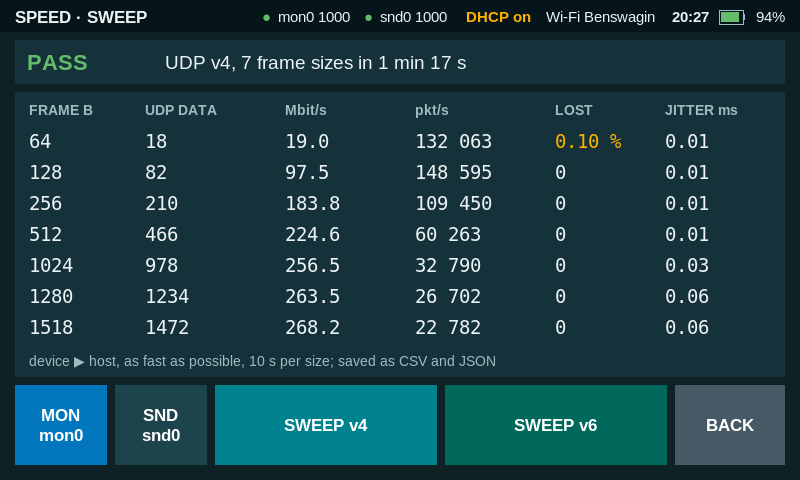
\includegraphics[width=0.72\textwidth]{Figures/gui_sweep.png}
    \caption{Výsledek rozmítání velikostí rámce na displeji přístroje}
    \label{fig:gui_sweep}
\end{figure}

Režim serveru byl ověřen tak, že měření spustil notebook proti přístroji (viz Obrázek \ref{fig:gui_server}). Přístroj přijal 249~Mbit/s protokolem TCP a v opačném směru odeslal 272~Mbit/s. Po stisku tlačítka STOP již v jmenném prostoru portu žádný proces serveru nezůstal.

\begin{figure}[htbp]
    \centering
    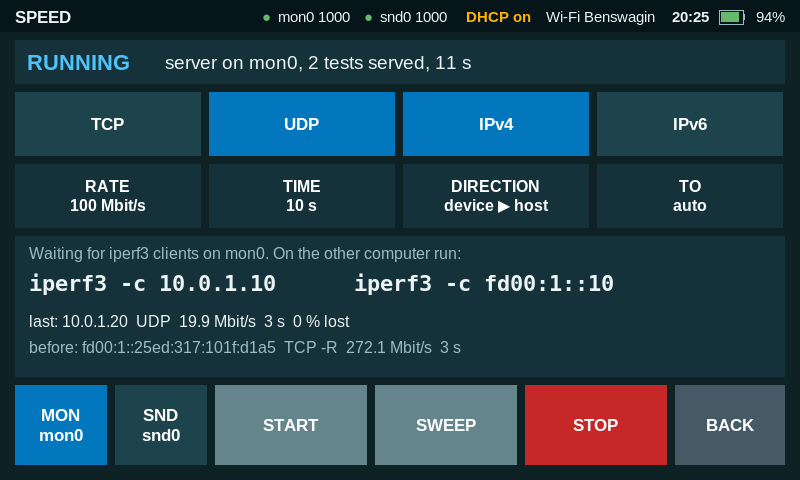
\includegraphics[width=0.72\textwidth]{Figures/gui_server.png}
    \caption{Režim serveru: notebook měří propustnost proti analyzátoru}
    \label{fig:gui_server}
\end{figure}

\subsection{Připojení běžného počítače}
\label{sec:overeni_notebook}

Notebook se systémem Windows 11 obdržel od přístroje na obou adaptérech adresy \texttt{10.0.1.20} a \texttt{10.0.2.20} a pro protokol IPv6 vždy tři adresy: adresu přidělenou serverem DHCPv6, adresu sestavenou bezstavově s identifikátorem neodvozeným z fyzické adresy a navíc dočasnou adresu. Výchozí trasa přes analyzátor nevznikla a notebook zůstal připojen k Internetu přes Wi-Fi, což potvrdilo správnost řešení popsaného v podkapitole \ref{sec:architektura}.

První test ping skončil bez odpovědi. Systém Windows považuje neznámou síť za veřejnou a příchozí zprávy Echo Request na ní blokuje; na zprávy zaslané na skupinovou adresu všech uzlů neodpovídá vůbec. Přístroj přitom správně ohlásil, že stanice je připojena, protože odpověděla na dotaz ARP i Neighbor Solicitation, a že ping blokuje její firewall. Po povolení příchozích zpráv Echo Request na obou testovacích adaptérech proběhly testy ze všech čtyř kombinací portu a protokolu bez ztráty s dobou odezvy 1,2 až 1,8~ms.

Měření protokolem UDP nad IPv6 se zpočátku nedařilo navázat. Záznam serveru iperf3 na notebooku ukázal, že server odpovídá ze své dočasné adresy, přestože analyzátor posílal požadavek na adresu přidělenou serverem DHCPv6. Dočasné adresy slouží k ochraně soukromí a systém jim při odesílání dává přednost \cite{rfc8981}; server iperf3 na adresu nevázaný tak odpověděl z jiné adresy, než na kterou byl osloven, a analyzátor takovou odpověď oprávněně zahodil. Po spuštění serveru vázaného na konkrétní adresu proběhlo měření bez chyby. Přístroj nyní v této situaci zobrazí vysvětlení i doporučení.

Nejvýznamnějším zjištěním bylo chování přenosu protokolem UDP v opačném směru, tedy z notebooku do analyzátoru. Při rychlosti 20~Mbit/s nebyly ztráty téměř žádné, při 50~Mbit/s činily 24~\% a při 100~Mbit/s 57~\%, přestože v témže směru přenesl protokol TCP 250~Mbit/s. Vyrovnávací paměť soketu na analyzátoru nepřetekla a notebook podle svých čítačů odeslal všechny datagramy. Rozhodl až čítač chybějících rámců adaptéru: během jednoho měření vzrostl o 13\,559, zatímco iperf3 napočítal 13\,543 ztracených datagramů. Rámce tedy zahazuje sám adaptér analyzátoru. Nástroj iperf3 v systému Windows sice dodržuje zadanou průměrnou rychlost, ale datagramy vysílá v dávkách plnou rychlostí gigabitové linky, a adaptér na sběrnici USB 2.0 je nestihne předat dál. Protokol TCP se této situaci přizpůsobí řízením toku, protokol UDP nikoli. Jde o skutečnou mez přístroje jako přijímače: dávkový provoz s rychlostí nad kapacitu sběrnice ztrácí už na vstupu. Přístroj proto nyní hodnotu tohoto čítače zaznamenává ke každému měření a vysvětlí, kde ke ztrátě došlo.

\subsection{Napájení a výdrž}
\label{sec:overeni_napajeni}

Výdrž přístroje byla změřena vybíjecí zkouškou v typickém provozu, tedy s pasivním odposlechem na monitorovacím portu, zapnutým displejem a připojenou sítí Wi-Fi. Přístroj pracoval z plně nabitého akumulátoru 6 hodin a 43 minut, než napětí článků kleslo pod 9,6~V a služba jej řádně vypnula (viz Obrázek \ref{fig:graf_vybijeni}). Akumulátor za tu dobu odevzdal 2,51~Ah a 28,2~Wh, tedy 84~\% jmenovité kapacity článků, při průměrném odběru 4,2~W. Napětí klesalo téměř rovnoměrně, s výjimkou poslední půlhodiny, kdy klesalo dvojnásobnou rychlostí. Nejhorší případ z Tabulky \ref{tab:spotreba} samostatně změřen nebyl; ze stejné energie a vyššího odběru vychází odhad přibližně čtyř hodin.

\begin{figure}[htbp]
    \centering
    % Vybijeci zkouska akumulatoru 3S, typicky provoz (pasivni odposlech), 25.-26.09.2026
\begin{tikzpicture}
    \begin{axis}[
        width=0.8\textwidth, height=5.8cm,
        xlabel={doba provozu z akumulátoru [h]},
        ylabel={napětí článků v sérii [V]},
        xmin=0, xmax=7, ymin=9.4, ymax=12.6,
        xtick={0,1,2,3,4,5,6,7},
        grid=major, grid style={gray!25},
        tick label style={font=\footnotesize}, label style={font=\small}]
        \addplot[thick] table[x=h, y=v] {Figures/data/discharge.csv};
        \draw[dashed] (axis cs:0,9.6) -- (axis cs:7,9.6);
        \node[anchor=south west, font=\footnotesize] at (axis cs:0.1,9.6) {práh vypnutí 9,6 V};
        \node[anchor=south west, font=\footnotesize, align=left] at (axis cs:0.3,10.05) {vypnutí po 6~h 43~min\\odevzdáno 28,2~Wh};
    \end{axis}
\end{tikzpicture}

    \caption{Napětí akumulátoru během vybíjecí zkoušky v typickém provozu}
    \label{fig:graf_vybijeni}
\end{figure}

Z téhož záznamu byla sestavena křivka, podle níž přístroj převádí napětí na zbývající náboj v procentech a odhaduje zbývající dobu provozu. Samostatně bylo změřeno, co ušetří uzamčení obrazovky: vypnutí výstupu HDMI snížilo odběr akumulátoru ze 4,53~W na 4,18~W, tedy o 0,35~W, což prodlouží výdrž uzamčeného přístroje zhruba o půl hodiny. Vypnutí linek testovacích portů nesnížilo odběr vůbec.

\subsection{Skenování sítě a ověření izolace jmenných prostorů}
\label{sec:skenovani}

Skener Nmap se spouští z obrazovky SCAN, a to buď přes testovací port uvnitř jeho jmenného prostoru, nebo přes rozhraní Wi-Fi s automatickým dosazením výchozí brány bezdrátové sítě. Obrázek \ref{fig:gui_nmap_lan} zachycuje sken druhého portu téhož přístroje přes propojku. Skener stanici nalezl, určil výrobce jejího adaptéru podle fyzické adresy a zjistil, že ze sta nejběžnějších portů není otevřen žádný; přístroj tedy na svých testovacích portech nevystavuje žádnou službu.

\begin{figure}[htbp]
    \centering
    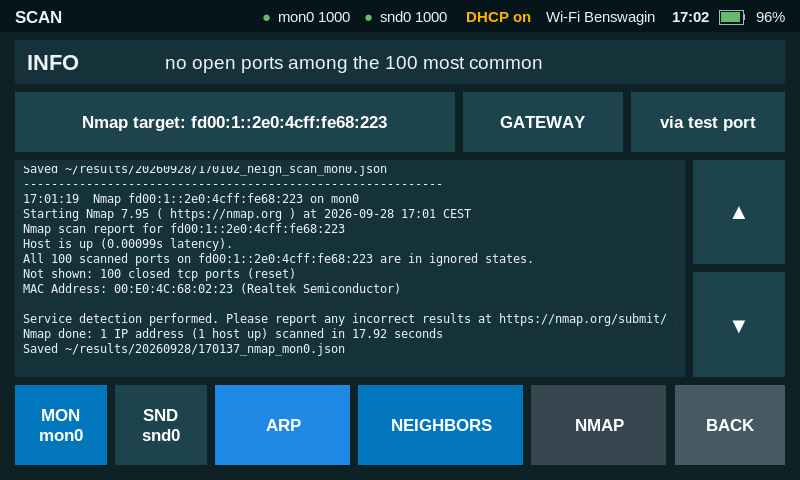
\includegraphics[width=0.72\textwidth]{Figures/gui_nmap_lan.png}
    \caption{Skenování nástrojem Nmap přes testovací port}
    \label{fig:gui_nmap_lan}
\end{figure}

Testování skeneru odhalilo i vadu první verze aplikace, která je zároveň dokladem izolace. Skener byl v režimu kabelového skenování spouštěn napevno ve jmenném prostoru \texttt{analyzer\_\allowbreak sender}, takže pokus o sken adresy \texttt{10.0.1.20} z podsítě monitorovacího portu skončil hlášením \texttt{failed to determine route}. Táž adresa byla z prostoru \texttt{analyzer\_\allowbreak monitor} dostupná bez potíží. Nešlo tedy o poruchu sítě, nýbrž o důsledek toho, že mezi prostory záměrně neexistuje cesta: provoz z jednoho prostoru se do druhého nedostane ani tehdy, je-li o to výslovně požádáno. Nástroje se nyní spouštějí vždy ve jmenném prostoru portu zvoleného na obrazovce.

\subsection{Vady odhalené při opakovaném ověřování}
\label{sec:odhalene_vady}

Opakované ověřování odhalilo několik vad, které se neprojevily při prvním průchodu měřením a mohly zůstat skryté až do nasazení přístroje mimo laboratoř.

Nejzávažnější se týkala původního počítadla provozu. To rozlišovalo protokoly podle slov v textovém výpisu nástroje tcpdump, jenže řádky se segmenty TCP slovo \enquote{TCP} neobsahují. Při kontrolním měření napočítalo počítadlo nula segmentů TCP, zatímco současně uložený soubor jich obsahoval 1202; počty UDP a ICMP byly přitom správné. Vada byla odstraněna nahrazením počítadla analyzátorem popsaným v podkapitole \ref{sec:analyzator}, který čte binární hlavičky.

Inicializační skript při opakovaném spuštění v témže běhu systému selhal, protože se pokoušel přesunout rozhraní do nového jmenného prostoru dříve, než je jádro po zrušení starého prostoru vrátilo do výchozího. Vada zanikla s přechodem na službu, která prostory nevytváří znovu, ale pouze doplňuje, co chybí.

Další vada řídicí aplikace byla odhalena způsobem, který stojí za zaznamenání. Na snímku obrazovky se výpis jevil jako přerušovaný a část textu se zdvojovala, přestože obsah výpisu odečtený programově byl bezvadný. Příčinou bylo, že jednotlivé úlohy zapisovaly do prvků rozhraní přímo z vlastních vláken, což použitá knihovna nepřipouští a co v krajním případě vede k pádu aplikace. Zápis do prvků rozhraní je nyní odkládán do hlavního vlákna.

Dvě menší vady odhalilo až připojení skutečného počítače a pořizování snímků pro tuto práci. Záznamy o adresách přidělených serverem DHCP přetrvávají dvanáct hodin, a přístroj proto po odpojení notebooku zkoušel oslovit stanici, která už nebyla připojena; kandidáti na cíl se nyní ověřují znovu. Skener Nmap, který nestihl stanici prozkoumat v nastaveném časovém limitu, byl vyhodnocen jako sken bez otevřených portů; nyní je vyhodnocen jako nedokončený. Obecným poučením je, že výstup na displeji je třeba porovnávat s nezávisle získanými daty a nespoléhat na to, co je vidět.
 
\chapter{Závěr}
\label{sec:zaver}

Cílem této bakalářské práce bylo navrhnout a realizovat přenosné zařízení pro testování a monitorování počítačových sítí, které obsahuje generátor a analyzátor provozu protokolů IPv4 a IPv6 a umožňuje měřit parametry sítě, jako jsou zpoždění, propustnost a ztrátovost. Tento cíl byl splněn.

V teoretické části byla popsána problematika generování síťového provozu, včetně rozdílu mezi měřením v bitech a v rámcích za sekundu, doporučených velikostí rámce a výpočtu rozptylu zpoždění, a problematika monitorování sítí, včetně filtrování provozu v jádře, souhrnných statistik a mezí samotného zachytávání. Dále byla rozebrána adresace a automatická konfigurace protokolu IPv6 a technologie jmenných prostorů, na níž je přístroj postaven.

V praktické části vznikl prototyp založený na jednodeskovém počítači Raspberry Pi s dotykovým displejem, dvěma externími síťovými adaptéry a akumulátorovým modulem. Přístroj se po zapnutí spustí přímo do řídicí aplikace a v typickém provozu vydrží z akumulátoru 6 hodin a 43 minut. Obsahuje analyzátor provozu se souhrnnými statistikami, rozborem jednotlivých rámců, filtry vyhodnocovanými v jádře a ukládáním do formátu pcap, generátor paketů šesti typů, měření zpoždění testem ping a měření propustnosti, ztrátovosti a rozptylu zpoždění nástrojem iperf3 včetně rozmítání velikostí rámce a režimu serveru. Pro protokol IPv6 nabízí audit zpráv Router Advertisement a vyhledání sousedů s odvozením jejich adres.

Řešení bylo ověřeno měřením, a to jak na propojce mezi oběma porty přístroje, tak proti cizí stanici se systémem Linux a proti notebooku se systémem Windows. Analyzátor napočítal stejné počty rámců jako nezávislý přepočet uloženého souboru a jeho rozbor se shodoval s analyzátorem Wireshark. Generátor doručil všechny odeslané pakety do druhého jmenného prostoru. Propustnost protokolem TCP dosáhla proti notebooku 273 až 276~Mbit/s pro oba protokoly IP.

\section*{Vlastní přínos autora}
\addcontentsline{toc}{section}{Vlastní přínos autora}

Prvním přínosem je architektura přístroje, v níž jsou obě testovací rozhraní logicky oddělena jmennými prostory jádra Linux a každá měřicí funkce je samostatným skriptem, který běží v prostoru zvoleného portu a svůj výsledek předává řídicí aplikaci ve strojově čitelném tvaru. Oddělení odstraňuje konflikty ve směrování mezi dvěma rozhraními v témže segmentu a bylo ověřeno měřením: pokus o oslovení cíle z nesprávného prostoru končí nedostupností cesty a pakety generátoru se do druhého prostoru dostanou pouze kabelem. Každý výsledek se ukládá i s časem a kontrolním součtem použitého skriptu, takže je dohledatelné, jak vznikl.

Druhým přínosem je rozbor adresní autokonfigurace protokolu IPv6 na straně analyzátoru. Bylo prokázáno, že server dnsmasq při rozsahu zadaném jedinou adresou zhasíná u inzerovaného prefixu příznak A, a že doplněním klíčového slova \texttt{slaac} si jádro cílové stanice sestaví adresu samo, bez jakéhokoli procesu v uživatelském prostoru; kontrolní port v původním nastavení potvrdil, že jiná příčina se na výsledku nepodílela. Na tento rozbor navazuje modul auditu, který zprávu Router Advertisement rozebere, posoudí vůči požadavkům norem a rozliší vysílání vlastního portu, druhého portu téhož přístroje a cizího směrovače, a vyhledání sousedů, které na témže vedení ukázalo, že protokol IPv6 protistranu nalezne i tam, kde protokol IPv4 nenalezne nic.

Třetím přínosem je dvojice generátoru a analyzátoru provozu s ověřenou přesností a změřenými mezemi. Analyzátor zachytí bez ztráty přibližně 22\,500 rámců za sekundu, generátor vyšle až 84\,000 rámců za sekundu a obě meze jsou dány výkonem procesoru, nikoli objemem dat. Měření dále ukázalo, že na propojce mezi porty je propustnost poloviční, protože každý rámec projde sběrnicí USB dvakrát, a že adaptér přístroje zahazuje rámce protokolu UDP, přicházejí-li v dávkách rychlejších, než je sběrnice stihne předat. Tato zjištění vymezují, jak naměřená čísla vykládat.

Čtvrtým přínosem je pojetí zařízení jako samostatného přístroje. Přístroj pracuje z vlastního akumulátoru s měřením stavu nabití a řádným vypnutím při vybití, ovládá se prstem na odporovém displeji s ovládacími prvky dimenzovanými pro dotyk a po připojení do cizí sítě sám od sebe nic nevysílá. Připojené stanici přiděluje pouze adresu, nikoli výchozí bránu, takže jí nenaruší stávající připojení k Internetu. U testů, které selžou, vysvětluje obsluze příčinu a doporučí další postup.

\section*{Omezení a doporučení pro další vývoj}
\addcontentsline{toc}{section}{Omezení a doporučení pro další vývoj}

Hranice přístroje je třeba vymezit poctivě. Ethernetové rozhraní použité platformy je připojeno přes sběrnici USB 2.0, a přístroj proto dosáhne nejvýše zhruba 276~Mbit/s; je způsobilý ověřit funkčnost spoje, porovnat protokoly za shodných podmínek a odhalit hrubé závady, nikoli však certifikovat gigabitovou linku. Odstranění tohoto omezení by vyžadovalo přechod na novější generaci jednodeskového počítače s ethernetovým řadičem mimo sběrnici USB. Týká se to i příjmu dávkového provozu protokolem UDP a meze analyzátoru v rámcích za sekundu.

Pro další vývoj se nabízí několik směrů. Nejbližším je ochranná konstrukce, do níž budou všechny komponenty pevně namontovány; přístroj již pracuje z akumulátoru, ale jeho části jsou zatím volně propojeny. Druhým směrem je automatický test zásuvky jedním tlačítkem, který by po připojení do sítě ověřil linku, dostupnost serveru DHCP a směrovače IPv6, výchozí bránu a překlad jmen, jak to činí komerční testery. Dalšími směry jsou zjišťování vlastností portu, tedy dohodnuté rychlosti, údajů ohlašovaných protokoly pro zjišťování sousedních prvků a značek VLAN, dále zjišťování největší velikosti paketu průchodné cestou, export výsledků na paměťové médium a zpřesnění dotykového ovládání kalibrací odporového panelu. Modul auditu protokolu IPv6 naznačuje i směr bezpečnostní: kontroly ověřené v této práci na záměrně vadné zprávě by v provozní síti dokázaly odhalit nesprávně nastavený nebo neoprávněně připojený směrovač.


% Seznam literatury
\printbibliography[title={Literatura}, heading=bibintoc]

% Prilohy
\appendix
\chapter{Zdrojové kódy měřicích skriptů}
\label{sec:Appendix1}

Příloha obsahuje skripty, které vykonávají vlastní síťovou práci přístroje. Každý z nich je samostatným nástrojem spustitelným i z příkazové řádky ve jmenném prostoru zvoleného portu. Přehled všech souborů programového vybavení je uveden v Příloze \ref{sec:Appendix2}.

\section*{Příprava testovacích portů (setup\_network.sh)}
\lstinputlisting[language=bash, label=src:SetupNetwork, caption={Přesun portů do jmenných prostorů, nastavení adres a spouštění serveru dnsmasq}]{SourceCodes/setup_network.sh}

\section*{Analyzátor provozu (sniff\_stats.py)}
\lstinputlisting[language=python, label=src:SniffStats, caption={Zachytávání nástrojem tcpdump s filtrem BPF a výpočet statistik provozu}]{SourceCodes/sniff_stats.py}

\section*{Generátor paketů (pkt\_gen.py)}
\lstinputlisting[language=python, label=src:PktGen, caption={Sestavení rámců knihovnou Scapy a jejich odeslání zadanou rychlostí}]{SourceCodes/pkt_gen.py}

\section*{Měření propustnosti, ztrátovosti a rozptylu zpoždění (perf\_test.py)}
\lstinputlisting[language=python, label=src:PerfTest, caption={Řízení nástroje iperf3, rozmítání velikostí rámce a vyhodnocení výsledku}]{SourceCodes/perf_test.py}

\section*{Audit zpráv Router Advertisement (ra\_audit.py)}
\lstinputlisting[language=python, label=src:RaAudit, caption={Vyžádání, rozbor a posouzení zprávy Router Advertisement}]{SourceCodes/ra_audit.py}

\section*{Vyhledání sousedů protokolu IPv6 (neigh\_scan.py)}
\lstinputlisting[language=python, label=src:NeighScan, caption={Vyjmenování sousedů a odvození jejich adres postupem EUI-64}]{SourceCodes/neigh_scan.py}

\section*{Skenování protokolem ARP (arp\_scan.py)}
\lstinputlisting[language=python, label=src:ArpScan, caption={Vyhledání aktivních stanic v rozsahu adres portu}]{SourceCodes/arp_scan.py}

\chapter{Přehled programového vybavení přístroje}
\label{sec:Appendix2}

Programové vybavení je uloženo v adresáři \texttt{\textasciitilde/diploma\_project/} na paměťové kartě přístroje; systémové soubory jsou na obvyklých místech systému. Úplné zdrojové kódy všech souborů jsou součástí elektronické přílohy práce. Tabulka \ref{tab:soubory} uvádí jejich přehled; skripty otištěné v Příloze \ref{sec:Appendix1} jsou označeny hvězdičkou.

\begin{table}[htbp]
    \caption{Soubory programového vybavení přístroje}
    \label{tab:soubory}
    \centering
    \small
    \begin{tabular}{lp{9.5cm}}
        \hline
        Soubor & Účel \\
        \hline
        \multicolumn{2}{l}{\textit{Měřicí skripty, spouštěné ve jmenném prostoru portu}} \\
        \texttt{setup\_network.sh}* & příprava portů, jmenných prostorů a serveru dnsmasq \\
        \texttt{sniff\_stats.py}* & analyzátor provozu, statistiky a ukládání do formátu pcap a CSV \\
        \texttt{pktdecode.py} & rozbor hlaviček rámce bez knihovny Scapy, pro statistiky i pro rozbor po vrstvách \\
        \texttt{pkt\_gen.py}* & generátor paketů šesti typů \\
        \texttt{perf\_test.py}* & měření nástrojem iperf3 a rozmítání velikostí rámce \\
        \texttt{perf\_server.py} & server iperf3 na zvoleném portu \\
        \texttt{path\_test.py} & test dostupnosti a zpoždění nástrojem ping \\
        \texttt{targets.py} & společné vyhledání cíle a vysvětlení, proč cíl chybí \\
        \texttt{ra\_audit.py}* & audit zpráv Router Advertisement \\
        \texttt{neigh\_scan.py}* & vyhledání sousedů protokolu IPv6 \\
        \texttt{arp\_scan.py}* & skenování protokolem ARP \\
        \multicolumn{2}{l}{\textit{Řídicí aplikace}} \\
        \texttt{gui\_app.py} & hlavní obrazovka, spouštění úloh, uvítací a zamykací obrazovka \\
        \texttt{ui\_kit.py} & společný vzhled obrazovek, stavový řádek, tlačítka \\
        \texttt{screens.py} & obrazovky PATH, SCAN, IPv6, DHCP / RA a SYSTEM \\
        \texttt{traffic.py} & obrazovka TRAFFIC s rozborem rámce a filtry \\
        \texttt{generator.py} & obrazovka GENERATOR \\
        \texttt{speed.py} & obrazovka SPEED s rozmítáním a režimem serveru \\
        \texttt{results.py} & ukládání výsledků do souborů JSON \\
        \texttt{wifi\_dialog.py} & připojení k síti Wi-Fi a klávesnice na obrazovce \\
        \multicolumn{2}{l}{\textit{Systémové služby}} \\
        \texttt{port\_status.py} & sledování stavu portů a zápis do stavového souboru \\
        \texttt{ups\_monitor.py} & měření stavu akumulátoru a řádné vypnutí při vybití \\
        \texttt{analyzer-port@.service} & příprava portu při připojení adaptéru \\
        \texttt{10-analyzer-*.link} & stálá jména portů podle fyzické adresy \\
        \texttt{\textasciitilde/.xinitrc} & spuštění řídicí aplikace místo pracovní plochy \\
        \hline
    \end{tabular}
\end{table}


\end{document}
